%\def\R{$\textsf{R}$}
%\def\S{$\textsf{S}$}

%\renewcommand{\labelitemii}{$\circ$}
\newcommand{\sfa}{a}
\newcommand{\worst}{\mbox{\em worst}}
\newcommand{\best}{\mbox{\em best}}
\newcommand{\regret}{\mbox{\em regret}}
\newcommand{\opt}{\mbox{\em opt}}
\newcommand{\join}{\bowtie}
\newcommand{\lE}{\underline{E}}
\newcommand{\uE}{\overline{E}}
\newcommand{\heads}{{\it heads}}
\newcommand{\tails}{{\it tails}}

\newcommand{\A}{{\cal A}}
\newcommand{\B}{{\cal B}}
\newcommand{\C}{{\cal C}}
\newcommand{\D}{{\cal D}}
\newcommand{\E}{{\cal E}}
\newcommand{\F}{{\cal F}}
\newcommand{\G}{{\cal G}}
%\newcommand{\H}{{\cal H}}
\newcommand{\I}{{\cal I}}
\newcommand{\J}{{\cal J}}
\newcommand{\K}{{\cal K}}
%\newcommand{\L}{{\cal L}}
\newcommand{\M}{{\cal M}}
\newcommand{\N}{{\cal N}}
%\newcommand{\O}{{\cal O}}
\newcommand{\Ocal}{{\cal O}}
\newcommand{\Hcal}{{\cal H}}
\renewcommand{\P}{{\cal P}}
\newcommand{\Q}{{\cal Q}}
\newcommand{\R}{{\cal R}}
%\newcommand{\S}{{\cal S}}
\newcommand{\T}{{\cal T}}
\newcommand{\U}{{\cal U}}
\newcommand{\V}{{\cal V}}
\newcommand{\W}{{\cal W}}
\newcommand{\X}{{\cal X}}
\newcommand{\Y}{{\cal Y}}
\newcommand{\Z}{{\cal Z}}


\newcommand{\IR}{\mathbb{R}}
\newcommand{\dfn}{\begin{definition}}
\newcommand{\edfn}{\end{definition}}
\newcommand{\thm}{\begin{theorem}}
\newcommand{\ethm}{\end{theorem}}
\newcommand{\xam}{\begin{example}}
\newcommand{\exam}{\end{example}}
\newcommand{\inter}{\cap}
\newcommand{\union}{\cup}




\documentclass[t, 8pt, seriff]{beamer}


%\documentclass[a4paper,xcolor=svgnames]{beamer} 
\usepackage[portuguese]{babel}
\usepackage[utf8]{inputenc}
\usepackage{times}
\usepackage{amsmath,amsthm}
\usepackage{amssymb,latexsym}
\usepackage{graphics}
%\usepackage{graphicx}

\usepackage{multimedia}
% \usepackage{movie15}
\usepackage{media9}

\usetheme{default}
%\usetheme{Singapore}
%\usetheme{PaloAlto} 
\usetheme{Boadilla}
% other themes: AnnArbor, Antibes, Bergen, Berkeley, Berlin, Boadilla, boxes, CambridgeUS, Copenhagen, Darmstadt, default, Dresden, Frankfurt, Goettingen,
% Hannover, Ilmenau, JuanLesPins, Luebeck, Madrid, Maloe, Marburg, Montpellier, PaloAlto, Pittsburg, Rochester, Singapore, Szeged, boxes, default

\useoutertheme{infolines}
%\usefonttheme{serif}
% you can also specify font themes: default, professionalfonts, serif, structurebold, structureitalicserif, structuresmallcapsserif

%\definecolor{vermelho}{RGB}{100,30,40}
%\definecolor{vermelholys}{RGB}{132,158,139}
%\definecolor{vermelholyslys}{RGB}{173,190,177}
%\definecolor{vermelholyslyslys}{RGB}{214,223,216}


%\usecolortheme[named=vermelho]{structure}




 



%\documentclass[a4paper,xcolor=svgnames]{beamer} 
%\usepackage[brazil]{babel}
%\usepackage[latin1]{inputenc}
\usepackage{ragged2e}
\usepackage{bm}
\usepackage[T1]{fontenc}
%\usepackage{amsmath,amsthm,amsfonts,amssymb} 
\usepackage{multirow}
%\usetheme{CambridgeUS} 
%\setbeamercolor{normal text}{bg=white}
\usepackage {graphicx,color}

\usepackage{wrapfig} % inserir a figura ao lado do texto
\usepackage[dvips]{epsfig} % inserir figuras de extensao post script (ps)
\usepackage{textcomp}
% \usepackage{undertilde} % colocar o til abaixo do x
\usepackage{multicol} % cor na linha
\usepackage{tabularx}
\usepackage{rotating} %rotacionar figuras e tabelas


\usepackage{ragged2e}
%\justifying


\usepackage{tikz}
\usetikzlibrary{trees}


\newtheorem{lema}{Lema}
\newtheorem{defi}{Definição}
\newtheorem{teo}{Teorema}
\newtheorem{corol}{Corolário}
\newtheorem{prop}{Proposição}


\newtheoremstyle{Exercício}{}{}{\rm}{}{\bf $\bigstar$ }{:}{ }{} %% \scshape para mudar
\theoremstyle{Exercício}
\newtheorem{exer}{Exercício}

\theoremstyle{plain}
\newtheoremstyle{Exemplo}{}{}{\rm}{}{\bf $\rhd$ }{:}{ }{} %% \scshape para mudar
%o tamanho a maiusculo
\theoremstyle{Exemplo}
\newtheorem{exem}{Exemplo}

% 
% \theoremstyle{plain}
% \newtheoremstyle{Nota}{}{}{\rm}{}{\bf\scshape}{:}{ }{}
% \theoremstyle{Nota}
 \newtheorem{nota}{Nota}






%\setlength{\rightskip}{0pt}
%\setlength{\leftskip}{0pt}
%\setlength{\spaceskip}{0pt}
%\setlength{\xspaceskip}{0pt}



\newcommand{\fullpage}[1]{
\begin{frame}
 #1
\end{frame}
}


\setbeamersize{text margin left=3em, text margin right=3em}



\setbeamertemplate{theorems}[numbered]



\definecolor{links}{HTML}{2A1B81}
\hypersetup{colorlinks,linkcolor=,urlcolor=links}


\graphicspath{{./graphics/}} 			% path das figuras (recomendável)

\newcommand{\cor}[1]{ \{{#1}\}}


\title[Probabilidade]{  Probabilidade (PPGECD000000001) \\ \vspace{1cm}Programa de Pós-Graduação em Estatística e Ciência de Dados (PGECD) }
\author[ Raydonal Ospina 
%\textcopyright 
\ ]{
	%Probabilidade\\ 
	Sessão 6 \\
	${}$ \\
	Raydonal Ospina  }

\date[]{}

\institute[UFBA]{Departamento de Estatística\\
	Universidade Federal da Bahia\\
	Salvador/BA}


\usecolortheme[rgb={0,0.6,0.6}]{structure}



%%%%%%%%%%%%%%%%%%%%%%%%%%%%%%%%%%%%%%%%%%%%%%%%%%%%%%%%%%%%%%%%%%%%%%
\begin{document}
% \SweaveOpts{concordance=TRUE}
\begin{frame}
  \titlepage
\end{frame}


%
%\begin{frame}{Variável aleatória}
%
%O conceito de variável aleatória (v.a.) é um mecanismo que permite relacionar qualquer resultado de um experimento aleatório com uma medida
%numérica.
%
%\begin{defi}
%	Sejam $\left( \Omega ,\frak{F}\right) $ e $\left( \Omega ^{\prime },\frak{F}%
%	^{\prime }\right) $ espaços mensuráveis. Uma aplicação $X:\Omega
%	\rightarrow \Omega ^{\prime }$ se diz $\frak{F-F}^{\prime
%	}-$\textit{mensurável} se para cada $A\in \frak{F}^{\prime },$ a imagem inversa $$X^{-1}\left(
%	A\right) =\left\{
%	\omega :X\left( \omega \right) \in A\right\} \in \frak{F}.$$
%\end{defi}
%
%\begin{defi}
%	Se $\left( \Omega ^{\prime },\frak{F}^{\prime }\right) =\left( \mathbb{R},%
%	\frak{B}\right) $ então falamos de \textit{funções reais mensuráveis.}
%	Se o par $\left( \Omega ^{\prime },\frak{F}^{\prime }\right) =\left( \overline{%
%		\mathbb{R}},\overline{\frak{B}}\right) $, em que os reais estendidos são definidos por $\overline{\mathbb{R}}=%
%	\mathbb{R\cup }\left\{ -\infty ,\infty \right\} $ e a $\sigma$-álgebra associada a $\overline{\mathbb{R}}$ é
%	$$\overline{\frak{B}}:=\left\{ B,B\cup \left\{ \infty \right\} ,B\cup \left\{ -\infty ,\infty
%	\right\} :B\in \frak{B}\right\},$$ em que $\frak{B}$ é a $\sigma$-álgebra de Borel nos reais, então falamos de \textit{funções
%		num\'{e}ricas mensuráveis.}
%\end{defi}
%
%
%\end{frame}
%%=====================================================================
%
%%%=====================================================================
%\begin{frame}
%\begin{defi}[Variável aleatória]
%Se $(\Omega ,\frak{F},P)$ é um espaço de probabilidade e $(\Omega ^{\prime
%},\frak{F}^{\prime })$ é um espaço mensurável, então uma função $
%X:\Omega \rightarrow \Omega ^{\prime }$ chama-se $(\Omega ^{\prime },\frak{F}%
%^{\prime })-$\emph{variável aleatória} (v.a.) se $X$ é uma função
%$\frak{F-F}^{\prime }$-mensurável.
%\end{defi}
%
%\begin{prop}
%Seja $\left( \Omega ,\frak{F}\right) $ um espaço mensurável (por exemplo, um espaço de probabilidade) e seja $X$ uma
%função numérica (assume valores reais). As seguintes afirmações são equivalentes:
%
%\begin{enumerate}
%	\item  $X$ é $\frak{F-B}$-mensurável
%	
%	\item  Para cada n\'{u}mero real $c$, o conjunto $\left\{ \omega\in
%	\Omega :X(\omega)>c\right\} $ $\in \frak{F.}$
%	
%	\item  Para cada n\'{u}mero real $c$, o conjunto $\left\{ \omega\in
%	\Omega :X(\omega)\geq c\right\} $ $\in \frak{F.}$
%	
%	\item  Para cada n\'{u}mero real  $c$, o conjunto $\left\{ \omega\in
%	\Omega :X(\omega)<c\right\} $ $\in \frak{F.}$
%	
%	\item  Para cada n\'{u}mero real  $c$, o conjunto $\left\{ \omega\in
%	\Omega :X(\omega)\leq c\right\} $ $\in \frak{F}$.
%	
%	Além disso, quaisquer das afirmações acima implicam em:
%	
%	\item  Para cada n\'{u}mero real $c$, o conjunto $\left\{ \omega\in
%	\Omega :X(\omega)=c\right\} $ $\in \frak{F.}$
%\end{enumerate}
%\end{prop}
%
%
%
%\end{frame}
%%%=====================================================================
%%
%%
%%%=====================================================================
%\begin{frame}
%\begin{proof}
%	A prova da proposição anterior é relativamente simples.Lembre sempre de olhar para as imagens inversas dos conjuntos e  mostre que 1) $\Rightarrow$ 2) $\Rightarrow$ 3) $\Rightarrow$ 4) $\Rightarrow$ 5) $\Rightarrow$ 6) $\Rightarrow$ 1). Resolva como exercício.
%\end{proof}
%
%\begin{exem}
%Seja $(\Omega, {\cal F}, P)$ um espaço de probabilidade em que ${\cal F} = {\cal
%B}$ e seja $A\in \frak{F}$ fixo. A função indicadora de $A$, $I_{A}$ definida por
%\begin{equation*}
%I_{A}\left( \omega \right) =\left\{ 
%\begin{array}{c}
%1,\text{ se }\omega \in A \\ 
%0,\text{ se }\omega \notin A
%\end{array}
%\right.
%\end{equation*}
%é uma função $\frak{F-B}$ mensurável, i.e., $I_{A}\left( \omega \right)$ é uma
%variável aleatória. De fato, para $a\in \mathbb{R}$
%
%\begin{equation*}
%I_{A}^{-1}\left( \left( a,\infty \right) \right) =\left\{ \omega
%:I_{A}\left( \omega \right) >a\right\} =
%\begin{cases}
%\Omega, & \text{se} \ a<0, \\ 
%A, & \text{se} \  0\leq a\leq 1,\\ 
%\emptyset, &\text{se} \ a>1.
%\end{cases}
%\end{equation*}
%\end{exem}
%\end{frame}
%
%%
%%
%\section{Definição}
%\begin{frame}
%\frametitle{\textbf{Variáveis aleatória real}}
%\baselineskip=13pt
%\begin{block}{Motivação}
%	
%	Suponha que uma moeda é lançada cinco vezes. Qual é o número de
%	caras? Esta quantidade é o que tradicionalmente tem sido chamada de
%	{\em variável aleatória}. Intuitivamente, é uma variável porque seus
%	valores variam, dependendo da sequência de lançamentos da moeda
%	realizada; o adjetivo ``aleatória'' é usado para enfatizar que o seu
%	valor é de certo modo incerto. Formalmente, contudo, uma variável
%	aleatória não é nem ``aleatória'' nem é uma variável.
%\end{block}
%
%
%\begin{defi}
%	Seja $(\Omega,\A,P)$ um espaço de probabilidade. Uma função
%	$X:\Omega \rightarrow R$ é chamada de variável aleatória se para
%	todo evento Boreliano $B$, $X^{-1}(B)\in \A$.
%\end{defi}
%
%Por definição, temos que $X^{-1}(B)=\{\omega\in\Omega:X(\omega)\in
%B\}$ é o conjunto de elementos do espaço amostral cuja imagem segundo $X$ está em $B$.
%
%O próximo teorema prova que para determinar se uma dada função real $X$ é uma variável aleatória só precisamos checar que a imagem inversa de intervalos da
%forma $(-\infty,x]$ pertence à $\sigma$-álgebra $\A$.
%\end{frame}
%%
%%
%\begin{frame}
%%\frametitle{\textbf{Definição}}
%\baselineskip=13pt
%
%
%%\pagebreak
%
%\begin{teo}
%	\label{teo1}
%	Seja $(\Omega,\A)$ um espaço mensurável. Uma função real $X:\Omega
%	\rightarrow R$ é uma variável aleatória se e somente se
%	$$X^{-1}((-\infty,\lambda])=\{w:X(w)\leq \lambda\}\in \A, \forall \lambda\in R.$$
%\end{teo}
%
%Considere os seguintes Lemas para a sua demonstração
%
%\begin{lema}\label{lem1}
%	Seja $\B$ a $\sigma$-álgebra de Borel, então
%	$X^{-1}(\B)=\{X^{-1}(B):B\in \B\}$ é uma $\sigma$-álgebra de eventos
%	de $\Omega$.
%\end{lema}
%
%\end{frame}
%
%%%
%\begin{frame}
%
%
%\begin{proof}[Prova do lema \ref{lem1}]
% Considere os três postulados para uma $\sigma$-álgebra:
%\begin{enumerate}
%\item[(i)] $\Omega\in X^{-1}(\B)$.
%
%Como $R\in \B$, nós temos $X^{-1}(R)=\Omega\in X^{-1}(\B)$.
%
%\item[(ii)] Se $A\in X^{-1}(\B)$, então $A^c\in X^{-1}(\B)$.
%
%Suponha que  $A\in X^{-1}(\B)$, então existe $A'\in\B$ tal que $A=X^{-1}(A')$. Como $\B$ é uma $\sigma$-álgebra, temos que $(A')^c\in \B$. Logo, $X^{-1}((A')^c)\in X^{-1}(\B)$. Como
%$X^{-1}((A')^c)=(X^{-1}(A'))^c,$ temos que $A^c\in X^{-1}(\B)$.
%
%\item[(iii)] Se $A_1,A_2,\ldots \in X^{-1}(\B)$, então $\cup_{i=1}^{\infty} A_i\in X^{-1}(\B)$.
%
%Suponha que  $A_1,A_2,\ldots \in X^{-1}(\B)$, então existem $A'_1,A'_2,\ldots \in\B$ tais que $A_i=X^{-1}(A'_i)$ para $i\geq 1$. Como $\B$ é uma $\sigma$-álgebra, temos que $\cup_{i=1}^{\infty}A'_i\in \B$. Logo, $X^{-1}(\cup_{i=1}^{\infty}A'_i)\in X^{-1}(\B)$. Como $\cup_{i=1}^{\infty} X^{-1}(A'_i)=X^{-1}(\cup_{i=1}^{\infty} A'_i)$, temos que $\cup_{i=1}^{\infty} A_i\in X^{-1}(\B)$.
%\end{enumerate}
%%\eprv
%%
%\end{proof}
%
%\bigskip
%Dado qualquer classe de conjuntos $\C$, denotamos por $\sigma(\C)$ a
%menor $\sigma$-álgebra contendo $\C$. Desta forma se
%$\B'=\{(-\infty,\lambda]:\lambda\in R\}$, então $\B=\sigma(\B')$. O
%próximo lema prova um resultado semelhante ao do lema anterior,
%porém mais forte.
%\end{frame}
%%%
%%%
%\begin{frame}
%
%%\frametitle{\textbf{Prova do Teorema}}
%%\baselineskip=13pt
%%\begin{block}{}
%%
%
%
%
%\begin{lema} \label{lem2}
%$X^{-1}(\B)=\sigma(X^{-1}(\B'))$, isto é, a imagem inversa de
%eventos Borelianos é igual a menor $\sigma$-álgebra contendo as
%imagens inversas dos
%%eventos Borelianos.
%intervalos da forma $(\infty,\lambda]$, onde $\lambda\in R$.
%\end{lema}
%
%\begin{proof}[Prova do lema \ref{lem2}]
% De acordo com Lema~\ref{lem1}, $X^{-1}(\B)$ é uma
%$\sigma$-álgebra. Como $\B'\subseteq \B$, temos que
%$X^{-1}(\B')\subseteq X^{-1}(\B)$. Então, por definição de menor
%$\sigma$-álgebra, temos que $$\sigma(X^{-1}(\B'))\subseteq
%X^{-1}(\B).$$ 
%Para provar igualdade, definimos
%$$\F=\{B'\subseteq R:X^{-1}(B')\in \sigma(X^{-1}(\B'))\}.$$
%É fácil provar que $\F$ é uma $\sigma$-álgebra; nós omitimos os
%detalhes. Por definição, temos que $X^{-1}(\F)\subseteq
%\sigma(X^{-1}(\B'))$ e $\B'\subseteq \F$. Como $\F$ é uma
%$\sigma$-álgebra, $\B=\sigma(\B')\subseteq \F$. Portanto,
%$$X^{-1}(\B)\subseteq X^{-1}(\F)\subseteq
%\sigma(X^{-1}(\B')).$$	
%\end{proof}
%\end{frame}
%%
%%%
%%%
%\begin{frame}
%%\frametitle{\textbf{Prova do Teorema}}
%%\baselineskip=13pt
%%
%\begin{proof}[Prova do Teorema \ref{teo1}]
%Agora nós podemos provar o teorema \ref{teo1}. Suponha que
%$X^{-1}(\B')\subseteq \A$. Por definição de menor $\sigma$-álgebra,
%$$\sigma(X^{-1}(\B'))\subseteq \A.$$ Então, pelo Lema~\ref{lem2},
%$X^{-1}(\B)\subseteq \A$, o que implica que $X$ é uma variável
%aleatória.
%\end{proof}%
%
%De forma gera temos a seguinte definição
%
%\begin{defi}{(Evento aleatório):}
%	Seja $X$ uma variável aleatória definida sobre o espaço de probabilidade $(\Omega ,\frak{F} ,P)$ e com valores num espaço mensurável  $(\Omega^\prime ,\frak{F}^\prime).$ Definimos o evento aleatório como o conjunto
%	$$\cor{X \in B} = \cor{\omega \in \Omega : X(\omega) \in B }, \quad \text{para todo} \ B \in \frak{F}^\prime.$$
%\end{defi}
%em particular, a definição é válida para variáveis aleatórias reais, i.e., quando 
%$ (\Omega^\prime ,\frak{F}^\prime) =\left( \mathbb{R},%
%\frak{B}\right).$
%
%
%
%
%\end{frame}
%
%
%\begin{frame}
%
%
%\begin{exem}
%	Seja $(\Omega ,\frak{F} ,P)$ um espaço de probabilidade com $\frak{F} ={\cal P} (\Omega ). $ Neste caso, qualquer função $X$ a valores reais é uma variável aleatória. Prove!
%\end{exem}
%
%\begin{exem}
%	Um dado é lançado ao acaso uma vez. Neste caso o espaço amostral é $\Omega
%	=\left\{ 1,2,3,4,5,6\right\} $. Se observamos o  número da face obtida no lançamento podemos definir  a variável aleatória $X$ como:
%	\begin{center}
%		\begin{tabular}{cccl}
%			$X:$ & $\Omega $ & $\rightarrow $ & $\Bbb{R}$ \\
%			& $\omega$ & $\mapsto $ & $X\left( \omega\right) =\omega,$ \\ 
%		\end{tabular}
%	\end{center}
%	a qual atribui a cada elemento $\omega$ do espaço amostral $\Omega $ um 
%	número real $X\left( \omega\right) $ da seguinte forma
%	\begin{center}
%		\begin{tabular}{cccl}
%			$X:$ & $\Omega $ & $\rightarrow $ & $\Bbb{R}$ \\
%			& $1$ & $\mapsto $ & $X\left( 1\right) =1$ \\
%			& 2 & $\mapsto $ & $X\left( 2\right) =2$ \\
%			& 3 & $\mapsto $ & $X\left( 3\right) =3$ \\
%			& 4 & $\mapsto $ & $X\left( 4\right) =4$ \\
%			& 5 & $\mapsto $ & $X\left( 5\right) =5$ \\
%			& 6 & $\mapsto $ & $X\left( 6\right) =6$%
%		\end{tabular}
%	\end{center}
%	Logo, dizemos que a variável aleatória assume valores em $\ \ X\ \ =\left\{1,2,3,4,5,6\right\}.$
%\end{exem}
%
%%  
%\end{frame}
%%
%
%
%\begin{frame}
%%%\end{block}
%%
%\begin{block}{Probabilidade Induzida}
%Dada uma variável aleatória $X$, pode-se definir uma probabilidade
%induzida $P_X$ no espaço mensurável $(R,\B)$ da seguinte maneira:
%para todo $A\in \B$, definimos $P_X(A)=P(X^{-1}(A))$. Por definição
%de variável aleatória, tem-se que $X^{-1}(A)\in \A$, então $P_X$
%está bem definida. Resta provar que $P_X$ satisfaz os axiomas K1,
%K2, e K4$'$ de probabilidade:
%\end{block}
%
%De forma geral, temos a seguinte definição
%
% \begin{defi}{(Distribuição da variável aleatória).} Seja $X:(\Omega ,\frak{F})\rightarrow (\Omega ^{\prime },\frak{F}^{\prime })$
%	uma aplicação mensurável e seja $P$ uma medida de probabilidade definida sobre
%	$\Omega .$ Então a função $$P_{X}(B)=P(\cor{X \in B})=P\left( X^{-1}(B)\right) =
%	P\left(\omega\in\Omega: X(\omega)\in B\right),$$ em que $B\in \frak{F}^{\prime },$ define
%	uma medida de probabilidade sobre $\Omega ^{\prime }.$  A medida $P_{X}$ chama-se \textit{\bf medida transportada ou induzida por }$X$ ou, simplesmente, a distribuição da
%	variável aleatória $X,$ já o conjunto  $\cor{X \in B}$ é o {\it evento aleatório.}
%\end{defi}
%
%
%\end{frame}
%
%\begin{frame}
%
%\begin{block}{Axiomas}
%	
%	\begin{enumerate}
%		\item[K1.] $P_X(A)=P(X^{-1}(A))\geq 0$.
%		\item[K2.] $P_X(R)=P(X^{-1}(R))=P(\Omega)=1$.
%		\item[K4.$\!'$] Suponha que $A_1, A_2, \ldots$ são eventos Borelianos
%		disjuntos. Então,
%		\begin{eqnarray}
%		& & P_X(\cup_i A_i)=P(X^{-1}(\cup_i A_i))=P(\cup_i X^{-1}(A_i)) \nonumber \\
%		& & =\sum_i P(X^{-1}(A_i))=\sum_i P_X(A_i). \nonumber
%		\end{eqnarray}
%	\end{enumerate}
%\end{block}
%
%
%\begin{exem}
%	Seja $\Omega=\cor{1,2,3},$ ${\cal F} = \cor{\emptyset, \cor{1}, \cor{2,3},
%		\Omega}$ e $P$ dada por: $P(\emptyset)=0,$ $P( \cor{1})= 1/5,$
%	$P(\cor{2,3})=4/5$ e $P(\Omega)=1.$ Se
%	$\Omega^{\prime}=\cor{a,b},$ $\frak{F}^{\prime }={\cal P}(\Omega^{\prime})$ e 
%	$X:\Omega \rightarrow \Omega^{\prime}$ dada por 
%	$$
%	\begin{cases}
%	a,& \ \text{se}  \ \ \omega =1, \\
%	b, & \ \text{se} \ \ \omega =2 \ \text{ou}  \ \omega=3,
%	\end{cases}
%	$$
%	então, a distribuição $P_X$ de $X$ é dada por:
%	$P_X(\emptyset)=0,$ $P_X(\cor{a})=P( \cor{1})= 1/5,$
%	$P_X(\cor{b})=P(\cor{2,3})=4/5$ e $P(\Omega^{\prime})=1.$
%\end{exem}
%\end{frame}
%
%\begin{frame}
%\frametitle{\textbf{Função de Distribuição Acumulada}}
%%\baselineskip=13pt
%%\begin{block}{}
%%
%Para uma variável aleatória $X$, uma maneira simples e básica de
%descrever a probabilidade induzida $P_X$ é utilizando sua {\em
%função de distribuição acumulada}.
%%
%\begin{defi}
%A função de distribuição acumulada de uma variável aleatória $X$,
%representada por $F_X$, é definida por
%%
%$$F_X(x)=P_X((-\infty, x]), \forall x\in R.$$
%\end{defi}
%
%\begin{block}{Propriedades}
%
%A função de distribuição acumulada $F_X$ satisfaz as seguintes
%propriedades:
%\begin{enumerate}
%\item[F1.] Se $x\leq y$, então $F_X(x)\leq F_X(y)$.
%\end{enumerate}
%De fato
%\begin{eqnarray}
%& & x\leq y \Rightarrow (-\infty, x]\subseteq (-\infty, y] \nonumber \\
%& & \Rightarrow P_X((-\infty, x])\leq P_X((-\infty, y])\nonumber \\
%& & \Rightarrow F_X(x)\leq F_X(y).\nonumber
%\end{eqnarray}
%
%\end{block}
%\end{frame}
%%
%%
%
%
%
%\begin{frame}
%\begin{block}{}
%
%\begin{enumerate}
%\item[F2.] Se $x_n\downarrow x$, então $F_X(x_n)\downarrow F_X(x)$.
%\end{enumerate}
%De fato. Se $x_n\downarrow x$, então os eventos $(-\infty, x_n]$ são
%decrescentes e $\cap_n(-\infty, x_n]=(-\infty, x]$. Logo, pela
%continuidade da medida de probabilidade, tem-se que $P_X((-\infty,
%x_n])\downarrow P((-\infty, x])$, ou seja, $F_X(x_n)\downarrow
%F_X(x)$.
%\end{block}
%
%\begin{block}{}
%
%\begin{enumerate}
%\item[F3.] Se $x_n\downarrow -\infty$, então $F_X(x_n)\downarrow 0$, e se $x_n\uparrow \infty$, então $F_X(x_n)\uparrow 1$.
%\end{enumerate}
%De fato. Se $x_n\downarrow -\infty$, então os eventos $(-\infty, x_n]$ são
%decrescentes e $\cap_n (-\infty, x_n]=\emptyset$. Logo, pela
%continuidade da medida de probabilidade, tem-se que $P_X((-\infty,
%x_n])\downarrow P(\emptyset)$, ou seja, $F_X(x_n)\downarrow 0$.
%Similarmente, se $x_n\uparrow \infty$, então os eventos $(-\infty,
%x_n]$ são crescentes e $\cup_n (-\infty, x_n]=\IR$. Logo, pela
%continuidade da medida de probabilidade, tem-se que $P_X((-\infty,
%x_n])\uparrow P(\Omega)$, ou seja, $F_X(x_n)\uparrow 1$.
%
%\end{block}
%\begin{teo}
%\label{thm:acumula}
%Uma função real $G$ satisfaz F1--F3 se e somente se $G$ é uma
%distribuição de probabilidade acumulada.
%\end{teo}
%\end{frame}
%
%\begin{frame}
%%
%\begin{proof} Aprova de que se $G$ for uma distribuição de probabilidade
%acumulada, então $G$ satisfaz F1-F3 foi dada acima. A prova de que
%toda função real que satisfaz F1-F3 é uma função de probabilidade
%acumulada é complexa envolvendo o Teorema da Extensão de
%Carathéodory. Nós apresentamos aqui um esquema de como a prova é
%feita. Primeiro define-se $P_X((-\infty, x])=F_X(x)$,
%$P_X((x,\infty))=1-F_X(x)$, e $P_X((a,b])=F_X(b)-F_X(a)$. Com esta
%definição, considera-se a álgebra formada por união finita de
%intervalos e prova-se que $P_X$ é $\sigma$-aditiva nesta álgebra.
%Finalmente, aplica-se o Teorema da Extensão de Carathéodory para
%provar que $P_X$ pode ser estendida para todo evento Boreliano.
%\end{proof}
%
%\begin{nota}
%	%
%	
%	Uma função de distribuição pode corresponder a várias variáveis aleatórias no mesmo espaço de probabilidade $(\Omega,\A,P)$. Por exemplo, se $X$ tem uma distribuição normal com parâmetros 0 e 1, então por simetria é fácil ver que $-X$ também distribuição normal com parâmetros 0 e 1. Consequentemente, $F_X=F_{-X}$. No entanto, $P(X=-X)=P(X=0)=0$.
%\end{nota}
%\end{frame}
%%
%%%
%\begin{frame}
%%%\frametitle{\textbf{Propriedades}}
%%%\baselineskip=13pt
%%
%\bigskip
%Condição F2 significa que toda função distribuição de probabilidade
%acumulada $F_X$ é continua à direita. Ainda mais, como $F_X$ é
%não-decrescente e possui valores entre 0 e 1, pode-se provar que ela
%tem um número enumerável de descontinuidades do tipo salto. Pela
%continuidade à direita , o salto no ponto $x$ é igual a
%\begin{eqnarray}
%& & F_X(x)-F_X(x^-)=F_X(x)-\lim_{n\rightarrow
%	\infty}F(x-\frac{1}{n})\nonumber\\
%& & = P_X((-\infty,x]) - \lim_{n\rightarrow
%	\infty}P_X((-\infty,x-\frac{1}{n}])\nonumber\\
%& & =\lim_{n\rightarrow\infty}P_X((x-\frac{1}{n},x]).\nonumber
%\end{eqnarray}
%
%Como a sequência de eventos $(x-\frac{1}{n},x]$ é decrescente e
%$\cap_n (x-\frac{1}{n},x]=\{x\}$. Temos que $\{x\}$ é Boreliano e
%%
%$$P_X(x)=F_X(x)-F_X(x^-).$$
%%
%%%
%%%\end{block}
%\begin{teo}
%Seja $D$ o conjunto de pontos de descontinuidade da função de distribuição $F$. Então, $D$ é enumerável.
%\end{teo}
%
%\end{frame}
%%%
%%%
%%%\begin{frame}
%%%\frametitle{\textbf{Propriedades}}
%%%\baselineskip=13pt
%%%\begin{block}{}
%%%
%%%%
%%
%%%
%%%\end{block}
%%%\end{frame}
%%%
%%%
%%\begin{frame}
%%%\frametitle{\textbf{Propriedades}}
%%%\baselineskip=13pt
%%%\begin{block}{}
%%%
%
%%%\end{block}
%%%
%%%\end{frame}
%%%
%%%
%\begin{frame}
%%%\frametitle{\textbf{Prova do Teorema}}
%%%\baselineskip=13pt
%%%
%%%\begin{block}{}
%%%
%\begin{proof}
%Pela monotonicidade, temos que para todo $x\in\IR$, $F(x^-)\leq F(x)\leq F(x^+)$. Logo, $x\in D$ se, e somente se, $F(x^+)>F(x^-)$. Para $n=1,2,3,\ldots$ seja
%$$A_n=\{x:F(x^+)-F(x^-)>\frac{1}{n}\}.$$
%Então, $D=\union_{n=1}^{\infty}A_n$.
%Vamos verificar que todo $A_n$ contém menos que $n$ pontos e, portanto, é finito. Dessa forma, $D$ será enumerável.
%
%Por absurdo, suponha que exista $A_n$ que contém $n$ pontos. Assim, $A_n=\{x_1,x_2,\ldots,x_n\}$, onde $x_1<x_2<\cdots x_n$ e
%\begin{eqnarray}
%& & 0\leq F(x_1^-)\leq F(x_1^+)\leq F(x_2^-)\leq F(x_2^+)\leq \cdots \nonumber\\
%& & \cdots \leq F(x_n^-)\leq F(x_n^+)\leq 1. \nonumber
%\end{eqnarray}
%Então, temos $\sum_{k=1}^{n}[F(x_k^+)-F(x_k^-)]\leq 1$.
%Mas por definição do conjunto $A_n$, temos que $F(x_i^+)-F(x_i^-)>\frac{1}{n}$ para todo $x_i\in A_n$. Portanto,
%$\sum_{k=1}^{n}[F(x_k^+)-F(x_k^-)]>n\times \frac{1}{n}= 1$, absurdo. Logo, $A_n$ contém menos que $n$ pontos.
%\end{proof}
%%%
%%%\end{block}
%\end{frame}
%
%
%\begin{frame}
%
%\begin{exem}
%	Suponhamos que se atira ao acaso uma moeda corrente três vezes consecutivas. Neste caso $\Omega =\{Cara, Coroa\} \times \{Cara, Coroa\} \times \{Cara, Coroa\}.$ Definimos 
%	$$X= \text{``n\'{u}mero de caras obtidas''}.$$ Note que, $X=\{0, 1, 2, 3 \}.$ Então, a função de distribuição $F_{X}$ da variável aleatória $X$ está dada por
%	$$
%	F_{X}(x)=\begin{cases}
%	0, & \text{se } \ x<0, \\
%	\frac{1}{8}, &\text{se } \ 0\leq x<1, \\
%	\frac{1}{2}, &\text{se } \ 1\leq x<2, \\
%	\frac{7}{8}, & \text{se } \ 2\leq x<3, \\
%	1, & \text{se } \ x\geq 3.\\
%	\end{cases}
%	$$
%	\vspace{-1.2cm}
%\begin{figure}[!htb]
%	\begin{center}
%		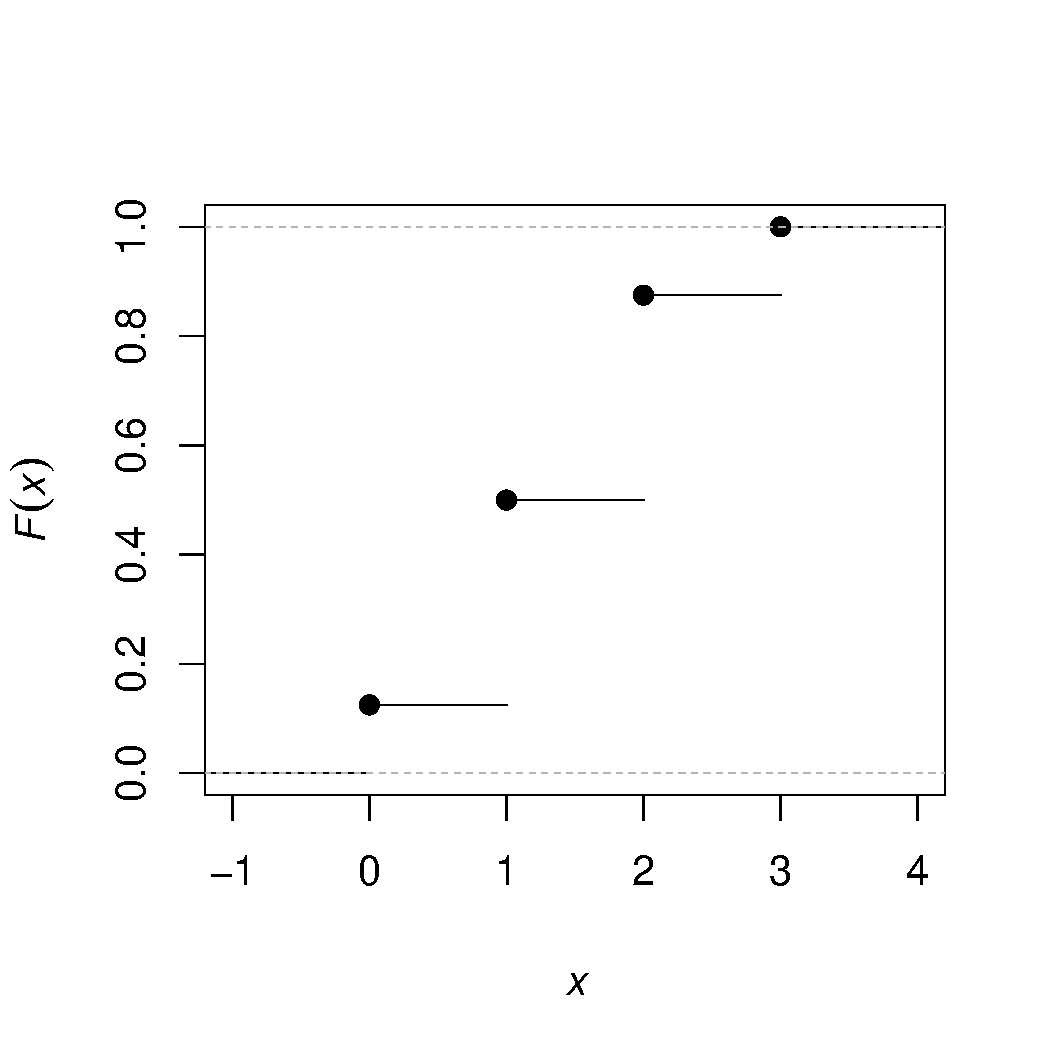
\includegraphics[scale=0.25]{fig11a.pdf}
%%		\caption{\label{fig11a} Representação gráfica da função de distribuição.}
%	\end{center}
%\end{figure}
%\end{exem}
%\end{frame}
%
%
%
%\begin{frame}
%
%\begin{exer}
%Da definição de função de distribuição podem ser obtidas as seguintes pro\-prieda\-des:
%	
%	\begin{enumerate}
%		
%		\item  $F(x^{-})={\lim_{_{0<h\rightarrow 0}} }F(x-h)=P(X<x).$
%		
%		\item $P(a\leq X\leq b)=F(b)-F(a^{-}).$
%		
%		\item $P(a<X\leq b)=F(b)-F(a).$
%		
%		\item $P(a\leq X<b)=F(b^{-})-F(a^{-}).$
%		
%		\item $P(a<X<b)=F(b^{-})-F(a).$
%		
%		\item $P(X=a)=F(a)-F(a^{-})$ ( deduz-se então que $F$ é contínua em $a,$ se e somente se, $P(X=a)=0$ ).
%		
%		\item Se $P(a<X<b)=0$ então $F$ é constante sobre o intervalo $(a,b).$
%		\end{enumerate}
%\end{exer}
%\end{frame}
%
%
%%
%\section{Tipos de Variável Aleatória}
%\begin{frame}
%\frametitle{\textbf{Tipos de Variável Aleatória}}
%%\baselineskip=13pt
%\begin{block}{Definição}
%Existem três tipos de variáveis aleatórias:
%\begin{itemize}
%\item {\bf Discreta.} Uma variável aleatória $X$ é {\em discreta} se assume um
%número enumerável de valores, ou seja, se existe um conjunto
%enumerável $\{x_1,x_2,\ldots\}\subseteq R$ tal que $X(w)\in
%\{x_1,x_2,\ldots\}, \forall w\in\Omega$. A função $p(x_i)$ definida
%por $p(x_i)=P_X(\{x_i\}), i=1,2,\ldots$ e $p(x)=0$ para $x\notin
%\{x_1,x_2,\ldots\}$, é chamada de {\em função probabilidade} de $X$. Note que neste caso, temos
%$$F_X(x)=\sum_{i:x_i\leq x}p(x_i).$$
%
%\item {\bf Contínua.} Uma variável aleatória $X$ é {\em contínua}  se
%existe uma função $f_X(x)\geq 0$ que é Riemman integrável tal que
%%
%$$F_X(x)=\int_{-\infty}^{x}f_X(t)dt, \forall x\in R.$$
%Neste caso, a função $f_X$ é chamada de {\em função densidade de
%probabilidade} de $X$.
%\item {\bf Singular.} Uma variável aleatória $X$ é {\em singular} se
%$F_X$ é uma função contínua cujos pontos de crescimento formam um
%conjunto de comprimento (medida de Lebesgue) nulo.
%\end{itemize}
%\end{block}
%
%\end{frame}
%
%%
%\begin{frame}
%Mais adiante veremos que pode-se decompor qualquer função de distribuição de probabilidade
%acumulada $F_X$ na soma de no máximo três
%funções de distribuição de probabilidade acumuladas, sendo uma
%discreta, uma contínua e outra singular.
%
%\begin{nota}{Para o caso de funções limitadas, se $f$ é uma função definida num intervalo $[a, b] \subset \mathbb{R}$ e
%		${\cal P} : a = x_0 < x_1 < \cdots < x_{n-1} < x_n = b$ é uma partição arbitrária de $[a, b].$ Dizemos que a função $f$ é Riemann integrável no intervalo $[a, b]$, se existir (e for finito) o limite seguinte:
%		$\lim_{ |{\cal P}|\rightarrow 0 }\sum_{i=1}^n f(\epsilon_i) \Delta x_i,$ independentemente da partição ${\cal P}$ do intervalo [$a, b],$  ou de como os pontos
%		$\epsilon_i$ pertencentes aos subintervalos $[x_{i-1} , x_i ]$ são escolhidos, em que $|{\cal P}|$ é o comprimento do maior intervalo contido na partição ${\cal P}$ e $\Delta x_i= x_i-x_{i-1}.$}
%\end{nota}
%
%%\end{block}
%\end{frame}
%%
%\begin{frame}
%\frametitle{\textbf{Variável Aleatória Discreta}}
%\baselineskip=13pt
%\begin{block}{}
%
%\begin{itemize}
%\item Se uma variável aleatória é
%discreta, então pode-se definir uma função de probabilidade $p$
%de modo que $p(x_i)=P_X(\{x_i\}), i=1,2,\ldots$, onde $X\subseteq
%\{x_1,x_2,\ldots\}$ e $p(x)=0$ para $x\notin \{x_1,x_2,\ldots\}$.
%Toda função de probabilidade é uma função dos reais $R$ e
%assume valores entre 0 e 1, sendo positiva para um número enumerável
%de pontos e satisfaz a seguinte propriedade $\sum_i p(x_i)=1$.
%
%
%\item Reciprocamente, dada uma função $p:R\rightarrow [0,1]$, onde $p$ é
%positiva para um número enumerável de pontos $\{x_1,x_2,\ldots\}$ e
%satisfaz $\sum_i p(x_i)=1$, uma função $P$ definida nos eventos
%Borelianos de modo que $P(A)=\sum_{x_i\in A}p(x_i), \forall A\in \B$
%é uma medida de probabilidade em $(R,\B)$ (verifique os axiomas de Kolmogorov!). Logo, a distribuição de uma variável aleatória
%discreta $X$ pode ser determinada tanto pela função de distribuição
%acumulada $F_X$ ou pela sua função de probabilidade $p$.
%\end{itemize}
%
%\end{block}
%
%\begin{exem}
%	Consideremos a variável aleatória $X$ que assume os valores 1,  2 e 3, com probabilidades 0,3, 0,5 e 0,2 respectivamente. Então a função de
%	probabilidade de $X$ é 
%	$$
%	p(x) =
%	\begin{cases}
%	0,3 & \text{se} \ x = 1, \\
%	0,5 & \text{se} \ x = 2, \\
%	0,2 & \text{se} \ x = 3, \\
%	0 & \text{caso contrário}.
%	\end{cases}
%	$$
%	cujo gráfico é indicado na Figura \ref{fig12}.
%	% Alternativamente, podemos expressar esta função através de uma tabela contendo as frequências. 
%	% \begin{center}
%	% \begin{tabular}{|c|c|c|c|} \hline
%	% $p(x)$ & 0,3 & 0,5 & 0,2  \\ \hline
%	% $x$ & 1 & 2 & 3 \\ \hline
%	% \end{tabular}
%	% \end{center}
%\end{exem}
%\end{frame}
%
%\begin{frame}
%\frametitle{\textbf{Variável Aleatória Contínua}}
%	\begin{figure}[!htb]
%	\begin{center}
%		\vspace{-0.5cm}
%		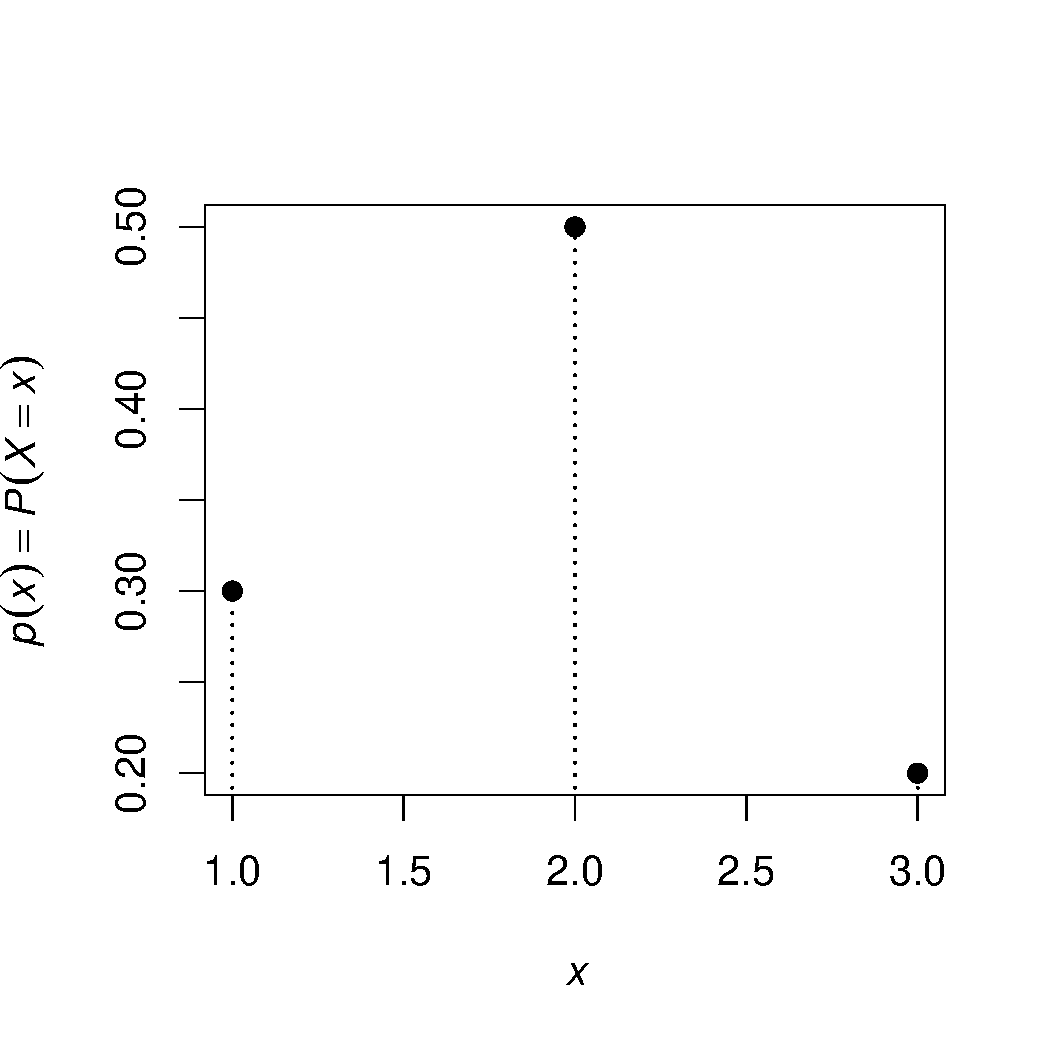
\includegraphics[scale=0.22]{fig12.pdf}
%				\vspace{-0.5cm}
%		\caption{\label{fig12} Representação gráfica da função de probabilidade $p(x).$}
%	\end{center}
%\end{figure}
%	\vspace{-0.2cm}
%\begin{block}{Variável Aleatória Contínua}
%
%Se uma variável aleatória é
%(absolutamente) contínua, então existe uma função $f_X(x)\geq 0$ tal
%que $F_X(x)=\int_{-\infty}^{x}f_X(t)dt$. Deste modo, $F_X$ é
%contínua e $f_X(x)=F'_X(x)$, exceto num conjunto de medida de
%Lebesgue nula. Uma função $f(x)\geq 0$ é densidade de alguma
%variável aleatória se e somente se,
%$\int_{-\infty}^{\infty}f(x)dx=1$, já que neste caso é fácil provar
%que a função $F$ definida por $\int_{-\infty}^{x}f(t)dt$ satisfaz as
%condições F1, F2, e F3, e portanto, pelo Teorema~\ref{thm:acumula} $F$
%é uma função de distribuição acumulada. Logo, a distribuição de uma
%variável aleatória contínua $X$ pode ser determinada tanto pela
%função de distribuição acumulada $F_X$ ou pela sua função de
%densidade $f_X$.
%
%\end{block}
%\end{frame}
%
%\begin{frame}
%%\frametitle{\textbf{Variável Aleatória Contínua}}
%%\baselineskip=13pt
%\begin{block}{}
%%
%%
%Uma variável aleatória $X$ tem densidade se $F_X$ é a integral (de
%Lebesgue) de sua derivada; sendo neste caso a derivada de $F_X$ uma
%função densidade para $X$. Este fato pode ser provado utilizando
%argumentos de Teoria da Medida. Sem
%recorrer a argumentos envolvendo Teoria da Medida, em quase todos os
%casos encontrados na prática, uma variável aleatória $X$ tem
%densidade se $F_X$ é (i) contínua e (ii) derivável por partes, ou
%seja, se $F_X$ é derivável no interior de um número finito ou
%enumerável de intervalos fechados cuja união é a reta $R$.
%%
%\end{block}
%
%No gráfico da Figura \ref{fig14} podemos observar a função de distribuição representada como a área embaixo da curva da função de densidade (painel esquerdo) e como uma função nos valores $x$ (painel direito).
%\begin{figure}[!htbp]
%	\vspace{-2.5cm}
%	\begin{center}
%		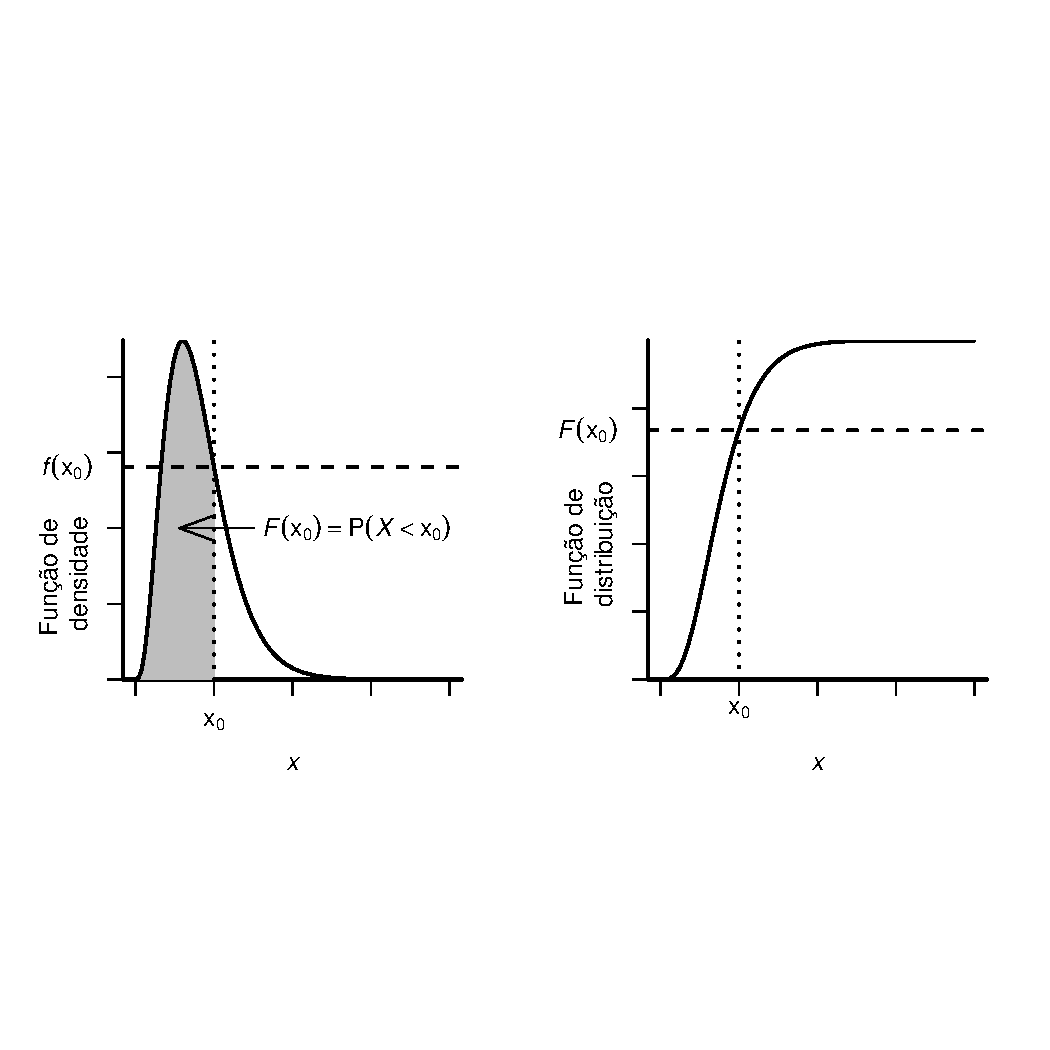
\includegraphics[scale=0.5]{fig14.pdf}
%		\vspace{-2.7cm}
%		\caption{\label{fig14} Representação gráfica de $f(x)$ e $F(x)$.}
%		
%	\end{center}
%\end{figure}
%
%\end{frame}
%%
%\begin{frame}
%\bigskip
%Das propriedades da $F(x)$ pode-se ver que
%\begin{equation*}
%2(\Delta x)f(x)\approx F(x+\Delta x)-F(x-\Delta x)=P(x-\Delta
%x<X\leq x+\Delta x)
%\end{equation*} isto é, a probabilidade de que $X$ esteja  num intervalo de comprimento pequeno ao redor de $x$ é igual a $f(x)$ pelo comprimento do intervalo.
%\begin{exem}
%Por exemplo, considere
%%
%\[
%F_X(x)= \left\{
%\begin{array}{ll}
%0 & \mbox{se \ $x< 0$,} \\
%x & \mbox{se \ $0\leq x< 1$,} \\
%1 & \mbox{se \ $x\geq 1$.}\\
%\end{array}
%\right.
%\]
%%
%Então $X$ tem densidade pois $F_X$ é contínua e derivável em todos
%os pontos da reta exceto em $\{0,1\}$.
%\end{exem}
%\end{frame}
%
%
%\begin{frame}
%\begin{exem} 
%	Seja $X$ uma variável aleatória contínua cuja função de distribuição é dada por: 
%	$$
%	F(x)=\begin{cases}
%	0\;\;&\text{se }x<0, \\
%	x&\text{se }0\leq x<1, \\
%	1&\text{se }x\geq 1.%
%	\end{cases}
%	\quad 
%	f(x)=\begin{cases}
%	1\;\;&\text{se}0\leq x\leq 1, \\
%	0&\text{caso contrário}%
%	\end{cases}
%	$$
%	é  uma função de densidade para $X$.
%\end{exem} 
%%  Para este exemplo, os gráficos de $f(x)$ e $F(x)$ aparecem na Figura \ref{fig15}.
%
%\begin{figure}[!htbp]
%	\vspace{-2.5cm}\begin{center}
%		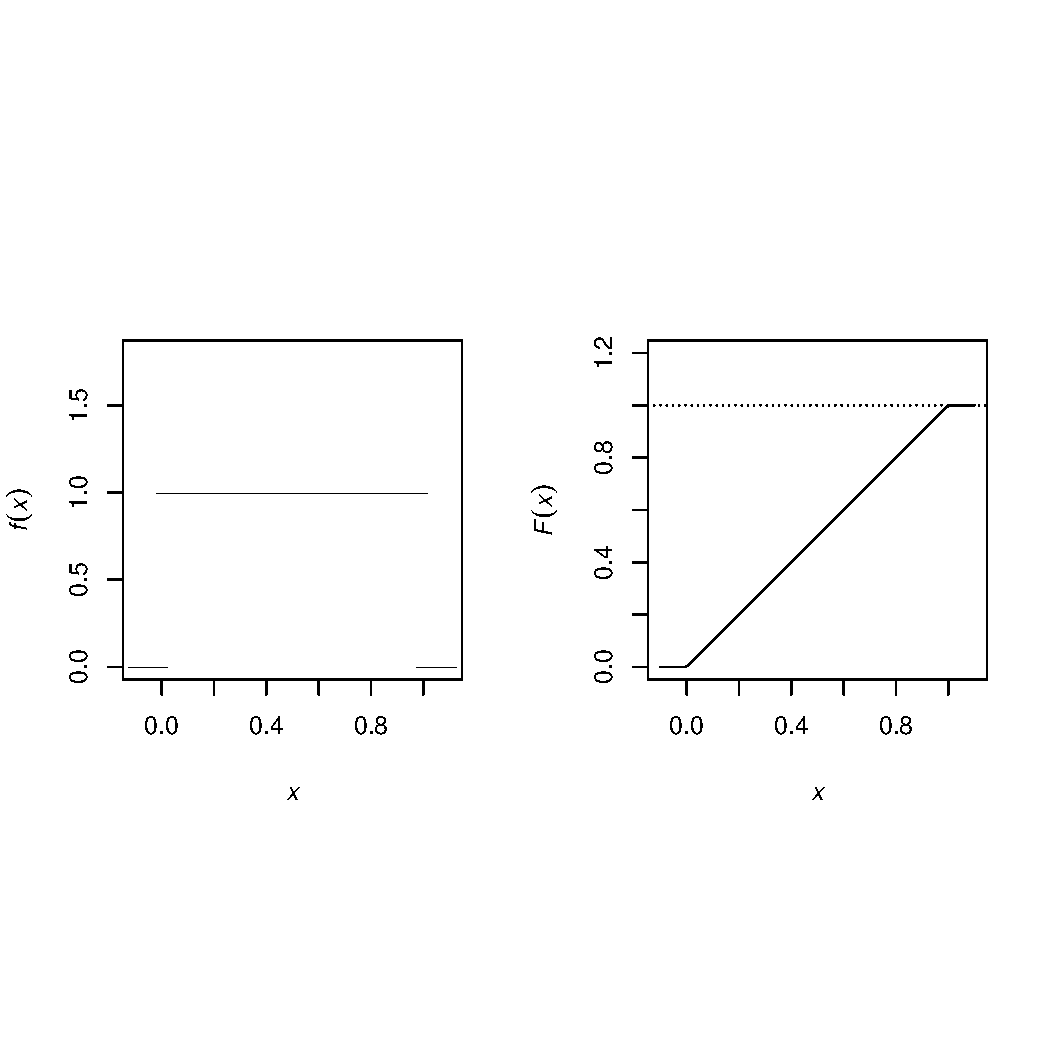
\includegraphics[scale=0.5]{fig15.pdf}\vspace{-2.3cm}
%		\caption{\label{fig15} Representação gráfica de $f(x)$ e $F(x)$.}
%	\end{center}
%\end{figure}
%\end{frame}
%%
%\begin{frame}
%\begin{block}{Variável Aleatória Singular}
%
%Vamos analisar um exemplo de uma função de distribuição de uma variável aleatória singular conhecida como {\em função de Cantor.} Esta função é contínua, derivável em todo ponto exceto em um conjunto de medida de Lebesgue nula, mas não é absolutamente contínua. Seja $F(x)=0$ se $x<0$ e $F(x)=1$ se $x>1$. Continuemos por etapas:
%
%\begin{description}
%\item[Etapa $1$:] Seja $F(x)=\frac{1}{2}$ para $x\in(1/3,2/3)$. Então, o valor de $F$ neste intervalo é igual a média dos valores de $F$ nos intervalos vizinhos em que $F$ já está definida: $(-\infty,0)$ e $(1,\infty)$. $F$ continua sem definição em dois intervalos: $[0,1/3]$ e $[2/3,1]$ de comprimento total 2/3.\\
%
%\item[Etapa $n+1$:] No terço central de cada um dos $2^n$ intervalos restantes após a etapa $n$, seja $F(x)$ igual à média dos valores nos dois intervalos vizinhos onde $F$ já está definida. Por exemplo, na etapa 2 defina $F(x)=1/4$ para $x\in(1/9,2/9)$ e $F(x)=3/4$ para $x\in\cup(7/9,8/9)$. Restarão então $2^{n+1}$ intervalos (o dobro do número restante após a etapa $n$), de comprimento total $(2/3)^{n+1}$, em que $F$ ainda não estará definida.
%\end{description}
%
%\end{block}
%\end{frame}
%%
%\begin{frame}
%%\frametitle{\textbf{Variável Aleatória Singular}}
%%\baselineskip=13pt
%\begin{block}{}
%%
%%
%Então definimos $F$ por indução em um número enumerável de intervalos abertos, cujo complementar (ou seja, o conjunto onde $F$ ainda não está definida) é o conjunto de Cantor, um conjunto de comprimento 0.
% 
%\medskip
%Podemos estender a definição de $F$ até o conjunto de Cantor $C$ por continuidade: se $x\in C$, a diferença entre os valores de $F$ nos dois intervalos vizinhos após a etapa $n$ é $1/2^n$.\\ 
%
%\medskip
%Note que $F$ é monótona não decrescente em $C^c$. Se $a_n$ é o valor de $F$ no intervalo vizinho esquerdo após a etapa $n$, e $b_n$ é o valor no intervalo vizinho direito após a etapa $n$, então, $a_n\uparrow$, $b_n\downarrow$ e $b_n-a_n\downarrow 0$. \\
%
%\medskip
%Seja $F(x)$ o limite comum de $a_n$ e $b_n$. Deste modo $F$ está definida em toda reta e é de fato uma função de distribuição (verifique!).\\
%
%\medskip
%Seja $X$ uma variável aleatória cuja função de distribuição é $F$, a função de Cantor. Então $X$ não é discreta e nem contínua pois $X$ não tem densidade $F'(x)=0$ em $C^c$ e $\int_{-\infty}^{x}F'(t)dt=0$, ou seja, $F$ não é a integral de sua derivada, ou melhor, não é absolutamente contínua. \\
%
%\medskip
%Como $F$ é contínua e $F'(x)=0$ para $x\in C^c$ e $C$ tem comprimento nulo, temos que $X$ é uma variável aleatória singular.
%
%\end{block}
%\end{frame}
%%
%\begin{frame}
%\begin{block}{Decomposição de uma Variável Aleatória}
%
%Seja $X$ uma variável aleatória qualquer e seja $F$ sua função de distribuição. Se $J=\{x_1,x_2,\ldots\}$ é o conjunto dos pontos de salto de $F$ (se $F$ for contínua $J=\emptyset$), indiquemos com $p_i$ o salto no ponto $x_i$, ou seja,
%$$p_i=F(x_i)-F(x_i^-).$$
%Definimos $F_d(x)=\sum_{i:x_i\leq x}p_i.$ $F_d$ é uma função degrau não-decrescente: a {\em parte discreta} de $F$. Como uma função monótona possui derivada em quase toda parte, seja
%%
%\[
%f(x)= \left\{
%\begin{array}{ll}
%F'(x) & \mbox{se $F$ é diferenciável em $x$,} \\
%0 & \mbox{se $F$ não é diferenciável em $x$.}\\
%\end{array}
%\right.
%\]
%
%\end{block}
%\end{frame}
%
%\begin{frame}
%
%\begin{block}{}
%
%
%Seja $F_{ac}(x)=\int_{-\infty}^{x}f(t)dt$. $F_{ac}$ é não-decrescente, pois a integral indefinida de uma função nao-negativa ($f\geq 0$ porque $F$ é não-decrescente). A sua derivada é igual a $f$ em quase toda parte, de modo que $F_{ac}$ é absolutamente contínua: $F_{ac}$ é a parte {\em absolutamente contínua} de $F$.
%
%Seja $F_s(x)=F(x)-F_d(x)-F_{ac}(x)$. $F_s$ é contínua pois é a diferença de duas funções contínuas. A derivada de $F_s$ é igual a zero em quase toda parte, porque $F$ e $F_{ac}$ têm a mesma derivada $f$, e $F_d$ possui derivada zero em quase toda parte. Pode-se provar que $F_s$ também é não-decrescente, mas está fora do escopo deste curso. $F_s$ é a {\em parte singular} de $F$.
%
%Esta discussão nos dá um método de decompor $F$ em suas partes discreta, absolutamente contínua e singular.
%
%\end{block}
%\end{frame}
%%
%\begin{frame}
%\begin{exem}
%
%%\begin{example}
%Suponha que $X\sim U[0,1]$ e $Y=min(X,1/2)$. Note que
%\[
%F_Y(x)= \left\{
%\begin{array}{ll}
%0 & \mbox{se $x<0$,} \\
%x & \mbox{se $0\leq x<1/2$,} \\
%1 & \mbox{se $x\geq 1/2$.}\\
%\end{array}
%\right.
%\]
%
%$F_Y$ tem apenas um salto em $x=1/2$ e $p_1=1/2$. Logo, $F_d(x)=0$ se $x<1/2$ e $F_d(x)=1/2$ se $x\geq 1/2$. Diferenciando $F_Y$, temos
%\[
%F'_Y(x)= \left\{
%\begin{array}{ll}
%0 & \mbox{se $x<0$ ou $x>1/2$,} \\
%1 & \mbox{se $0<x< 1/2$.}\\
%\end{array}
%\right.
%\]
%
%
%Logo, por definição,
%\[
%f(x)= \left\{
%\begin{array}{ll}
%0 & \mbox{se $x\leq 0$ ou $x\geq 1/2$,} \\
%1 & \mbox{se $0<x< 1/2$.}\\
%\end{array}
%\right.
%\]
%Portanto,
%\[
%F_{ac}(x)= \int_{-\infty}^{x}f(t)dt=\left\{
%\begin{array}{ll}
%0 & \mbox{se $x< 0$,} \\
%x & \mbox{se $0\leq x\leq 1/2$,} \\
%1/2 & \mbox{se $x> 1/2$.}\\
%\end{array}
%\right.
%\]
%Como $F_d+F_{ac}=F_Y$, temos que $F_s(x)=0$, $\forall x\in\IR$ e não há parte singular. {\em Uma variável aleatória que possui apenas partes discreta e absolutamente contínua é conhecida como uma variável aleatória mista.} Na prática, é pouco provável que surja uma variável aleatória singular. Portanto, quase todas as variáveis aleatórias são discretas, contínuas ou mistas.
%\end{exem}
%\end{frame}
%
%
%\begin{frame}
%\begin{exem}
%	Seja $X$ a variável aleatória com função de distribuição dada por:%
%	\begin{equation*}
%	F(x)=
%	\begin{cases}
%	1-\frac{1}{2}e^{-\lambda x}&\text{se }x\geq 0, \\
%	0&\text{caso contrário},%
%	\end{cases}
%	\end{equation*} 
%	em que $\lambda >0$ é uma constante.  A variável aleatória $X$ não  é discreta nem contínua pois apresenta um ponto de descontinuidade em $x=0.$ Ou seja é Singular. Para $\lambda=1/2$ o gráfico de $F(x)$ é apresentado na seguinte figura. %\ref{fig17}
%\end{exem}
%
%\begin{figure}[!htb]
%	%\vspace{-3cm}
%	\begin{center}
%		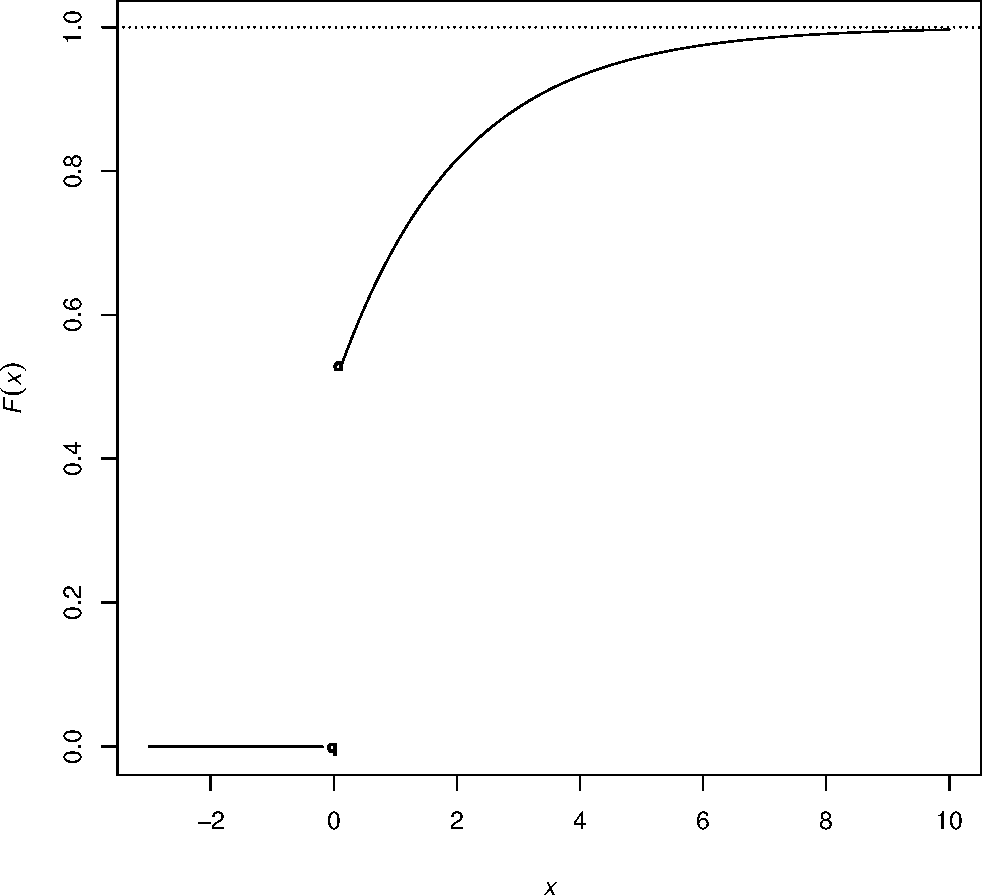
\includegraphics[scale=0.26]{fig17.pdf}
%		% \vspace{-1.5cm}
%		% \caption{\label{fig17} Representação gráfica de $F(x)$.}
%		
%	\end{center}
%\end{figure}
%
%\end{frame}
%
%
%
%
%
%\section{Principais Distribuições}
%\begin{frame}
%\frametitle{\textbf{Principais Distribuições Discretas}}
%\baselineskip=13pt
%\begin{block}{Aleatória - Uniforme discreta}
%
%$X$ tem uma distribuição {\em
%aleatória} com parâmetro $n$, onde $n$ é um número inteiro, se
%$X(w)\in \{x_1,x_2,\ldots,x_n\}$ e $p(x_i)=\frac{1}{n}$, para
%$i\in\{1,\ldots,n\}$.
%\begin{itemize}
%\item Utilizando a propriedade de aditividade da
%probabilidade, é fácil ver que para qualquer evento\\ $A\subseteq
%\{x_1,x_2,\ldots,x_n\}$, temos que $P(X\in A)=\frac{||A||}{n}$.
%
%\item Aplicações: modelar
%mecanismos de jogos (dados e moedas balanceados, cartas
%bem embaralhadas).
%\end{itemize}
%
%\end{block}
%\end{frame}
%
%\begin{frame}
%\frametitle{\textbf{Principais Distribuições  Discretas}}
%\baselineskip=13pt
%\begin{block}{Bernoulli}
%
%$X$ tem uma distribuição {\em
%Bernoulli} com parâmetro $p$, onde $0\leq p\leq 1$, se $X(w)\in
%\{x_0,x_1\}$ e $p(x_1)=p=1-p(x_0)$.
%
%
%\begin{itemize}
%\item Aplicações: modelar
%a probabilidade de sucesso em uma única realização de um
%experimento. Em geral, qualquer variável aleatória dicotômica pode ser modelada por uma distribuição Bernoulli.
%\end{itemize}
%
%\end{block}
%\end{frame}
%
%\begin{frame}
%\frametitle{\textbf{Principais Distribuições Discretas}}
%\baselineskip=13pt
%\begin{block}{Binomial}
%
%$X$ tem uma distribuição {\em
%Binomial} com parâmetros $n$ e $p$, onde $n$ é um número inteiro e
%$0\leq p\leq 1$, se $X(w)\in \{0,1,\ldots,n\}$ e
%$p(k)=\binom{n}{k}p^k(1-p)^{1-k}$, para $k\in\{0,1,\ldots,n\}$.
%
%Note que utilizando o Teorema Binomial, temos que
%$$\sum_{k=0}^{n}p(k)=\sum_{k=0}^{n}\binom{n}{k}p^k(1-p)^{n-k}=(p+1-p)^n=1.$$
%Logo, esta é uma legítima função probabilidade de massa.
%
%\end{block}
%\end{frame}
%
%\begin{frame}
%\frametitle{\textbf{Principais Distribuições Discretas}}
%\baselineskip=13pt
%\begin{block}{Binomial (cont.)}
%
%\begin{itemize}
%\item Pode-se provar que a soma de $n$ variáveis aleatórias Bernoulli com parâmetro $p$ independentes tem uma distribuição $Binomial(n,p)$.
%
%\item Aplicações: modelar a
%quantidade de erros em um texto de $n$ símbolos quando os erros
%entre símbolos são assumidos independentes e a probabilidade de erro
%em um símbolo do texto é igual a $p$; modelar o número de caras em $n$ lançamentos de uma moeda que possui
%probabilidade $p$ de cair cara em cada lançamento. Se $p=1/2$, temos
%um modelo para o número de 1's em uma sequência binária de
%comprimento $n$ escolhida aleatoriamente ou o número de caras em $n$
%lançamentos de uma moeda justa.
%\end{itemize}
%
%\end{block}
%\end{frame}
%%
%\begin{frame}
%\frametitle{\textbf{Principais Distribuições Discretas}}
%\baselineskip=13pt
%\begin{block}{Geométrica}
%
%$X$ tem uma distribuição {\em
%Geométrica} com parâmetro $\beta$, onde $0\leq \beta <1$, se
%$X(w)\in \{0,1,\ldots\}$ e $p(k)=(1-\beta)\beta^k$, para
%$k\in\{0,1,\ldots\}$.
%
%Utilizando o resultado de uma soma infinita de uma Progressão
%Geométrica, temos que
%$$\sum_{k=0}^{\infty}p(k)=\sum_{k=0}^{\infty}(1-\beta)\beta^k=(1-\beta)\sum_{k=0}^{\infty}\beta^k=1.$$
%Logo, esta é uma legítima função probabilidade de massa.
%
%\begin{itemize}
%\item Aplicações: modelar
%o tempo de espera medido em unidades de tempo inteira até a chegada
%do próximo consumidor em uma fila, até a próxima emissão de um
%fóton, ou até a primeira ocorrência de cara numa sequência de
%lançamentos de uma moeda.
%\end{itemize}
%
%\end{block}
%\end{frame}
%%
%\begin{frame}
%\frametitle{\textbf{Principais Distribuições Discretas}}
%\baselineskip=13pt
%\begin{block}{Binomial Negativa ou Pascal}
%
%É uma generalização da distribuição
%geométrica. Suponha que ao invés de estarmos interessados no tempo
%de espera até a primeira ocorrência de um evento, estejamos
%interessados em calcular o tempo de espera até a $r$-ésima
%ocorrência de um evento. Seja $Y$ o tempo de espera necessário a fim
%de que um evento $A$ possa ocorrer exatamente $r$ vezes. Temos que
%$Y=k$ se, e somente se, $A$ ocorrer na $(k+1)$-ésima repetição e $A$
%tiver ocorrido $r-1$ vezes nas $k$ repetições anteriores. Assumindo
%independência entre os experimentos, esta probabilidade é igual
%$p\binom{k}{r-1}p^{r-1}(1-p)^{k-r+1}$. Portanto,
%$$P(Y=k)=\binom{k}{r-1}p^{r}(1-p)^{k-r+1},\mbox{ onde }k\geq r-1.$$
%Note que se $r=1$, temos que $Y$ tem uma distribuição geométrica com
%parâmetro $\beta=1-p$. No caso geral, dizemos que $Y$ tem uma
%distribuição {\em Binomial Negativa ou Pascal}.
%
%\end{block}
%\end{frame}
%%
%\begin{frame}
%\frametitle{\textbf{Principais Distribuições Discretas}}
%\baselineskip=13pt
%\begin{block}{Relação entre as Distribuições Binomial e Binomial Negativa}
%
%
%Se $X\sim Binomial(n,p)$ e $Y\sim Pascal(r,p)$, então
%temos que $\{X\geq r\}=Y+1\leq n$, ou seja, o número de sucessos em
%$n$ repetições de um experimento é maior ou igual a $r$ se, e somente se, o tempo de
%espera para o $r$-ésimo sucesso for menor ou igual a $n-1$.
%Portanto,
%$$P(X\geq r)=P(Y\leq n-1).$$
%
%\end{block}
%\end{frame}
%
%\begin{frame}
%\frametitle{\textbf{Principais Distribuições Discretas}}
%\baselineskip=13pt
%\begin{block}{Relação entre as Distribuições Binomial e Binomial Negativa}
%
%
%Observe que estas duas distribuições tratam de experimentos
%repetidos.
%\begin{itemize}
%\item A distribuição binomial surge quando lidamos com um
%número fixo de experimentos e estamos interessados no número de sucessos
%que venham a ocorrer.
%\item A distribuição binomial negativa é encontrada
%quando fixamos o número de sucessos e então registramos o tempo de
%espera necessário.
%\end{itemize}
%
%\end{block}
%\end{frame}
%%
%\begin{frame}
%\frametitle{\textbf{Principais Distribuições Discretas}}
%\baselineskip=13pt
%\begin{block}{Zeta ou Zipf}
%
%$X$ tem uma distribuição Zeta
%ou Zipf com parâmetro $\alpha$, onde $\alpha>1$, se
%$X(w)\in\{1,2,\ldots\}$ e
%$$p(k)=\frac{k^{-\alpha}}{\zeta(\alpha)},k=1,2,\ldots,$$
%onde $\zeta(\alpha)=\sum_{k=1}^{\infty}k^{-\alpha}$ é conhecida como
%a função Zeta de Riemann.
%
%\begin{itemize}
%\item A função de probabilidade Zeta ou Zipf é um exemplo de uma
%distribuição de cauda pesada; observe que ela tem decaimento polinomial.
%
%\item Aplicações: número de consumidores afetados por um blackout, tamanhos
%de arquivos solicitados em transferência via Web e atraso de pacotes
%na internet.
%\end{itemize}
%
%\end{block}
%\end{frame}
%%
%\begin{frame}
%\frametitle{\textbf{Principais Distribuições  Discretas}}
%\baselineskip=13pt
%\begin{block}{Hipergeométrica}
%
%
%A distribuição hipergeométrica descreve o número de sucessos em uma
%sequência de $n$ amostras de uma população finita sem reposição.
%
%\medskip
%
%Considere que tem-se uma carga com $N$ objetos dos
%quais $D$ têm defeito. A distribuição hipergeométrica descreve a
%probabilidade de que em uma amostra de $n$ objetos distintos
%escolhidos da carga aleatoriamente exatamente $k$ objetos sejam
%defeituosos.
%
%\medskip
%
%Formalmente, se uma variável aleatória $X$ segue uma distribuição
%hipergeométrica com parâmetros  $N, D,$ e $n$, então a probabilidade de
%termos exatamente $k$ sucessos é dada por
%$$p(k)=\frac{\binom{D}{k}\binom{N-D}{n-k}}{\binom{N}{n}}.$$
%
%Esta probabilidade é positiva se: $N-D\geq n-k$, ou seja
%$k\geq\max(0,D+n-N)$, e $k\leq \min(n,D)$.
%
%
%\end{block}
%\end{frame}
%
%\begin{frame}
%\frametitle{\textbf{Principais Distribuições Discretas}}
%\baselineskip=13pt
%\begin{block}{Hipergeométrica (cont.)}
%
%
%%Esta fórmula pode ser entendida assim: existem $\binom{N}{n}$
%%possíveis amostras sem reposição. Existem $\binom{D}{k}$ maneiras de
%%escolher $k$ objetos defeituosos e existem $\binom{N-D}{n-k}$
%%maneiras de preencher o resto da amostra com objetos sem defeito.
%
%\begin{itemize}
%\item Quando a população é grande quando comparada ao tamanho da amostra
%(ou seja, $N$ for muito maior que $n$) a distribuição
%hipergeométrica é aproximada razoavelmente bem por uma distribuição
%binomial com parâmetros $n$ (tamanho da amostra) e $p = D / N$
%(probabilidade de sucesso em um único ensaio).
%
%\item Note que se a amostragem é feita com reposição, temos que a distribuição correta é dada por uma $Binomial(n,D/N)$.
%\end{itemize}
%
%\end{block}
%\end{frame}
%
%\begin{frame}
%\frametitle{\textbf{Principais Distribuições Discretas}}
%\baselineskip=13pt
%\begin{block}{Poisson}
%
%$X$ tem uma distribuição {\em
%Poisson} com parâmetro $\lambda$, onde $\lambda \geq 0$, se $X(w)\in
%\{0,1,\ldots\}$ e $p(k)=e^{-\lambda}\frac{\lambda^k}{k!}$, para
%$k\in\{0,1,\ldots\}$.
%
%Por definição, temos que para todo $x$ real,
%$$e^x=\sum_{k=0}^{\infty}\frac{x^k}{k!}.$$
%Utilizando este fato, temos que
%$$\sum_{k=0}^{\infty}p(k)=\sum_{k=0}^{\infty}\frac{e^{-\lambda}\lambda^k}{k!}=e^{-\lambda}\sum_{k=0}^{\infty}\frac{\lambda^k}{k!}=e^{-\lambda}e^{\lambda}=1.$$
%%Logo, esta é uma legítima função probabilidade de massa.
%
%\begin{itemize}
%
%\item Aplicações: modelar a
%contagem do número de ocorrências de eventos aleatórios em um certo
%tempo $T$, como número de fótons emitidos por uma fonte de luz de
%intensidade $I$ fótons/seg em $T$ segundos ($\lambda=IT$), número de
%clientes chegando em uma fila no tempo $T$ ($\lambda= C T$), número
%de ocorrências de eventos raros no tempo $T$ ($\lambda=C T$).
%
%\end{itemize}
%
%\end{block}
%\end{frame}
%%
%\begin{frame}
%\frametitle{\textbf{Principais Distribuições Discretas}}
%\baselineskip=13pt
%\begin{block}{Poisson como um Limite de Eventos Raros de Binomial}
%
%Suponhamos que chamadas telefônicas cheguem em uma grande central, e
%que em um período particular de três horas (180 minutos), um total
%de 270 chamadas tenham sido recebidas, ou seja, 1,5 chamadas por
%minuto. Suponhamos que queiramos calcular a probabilidade de serem
%recebidas $k$ chamadas durante os próximos três minutos.
%
%\medskip
%
%Ao considerar o fenômeno da chegada de chamadas, poderemos chegar à
%conclusão de que, a qualquer instante, uma chamada telefônica é tão
%provável de ocorrer como em qualquer outro instante. Como em
%qualquer intervalo de tempo, temos um número infinito de pontos,
%vamos fazer uma série de aproximações para este cálculo.
%
%\end{block}
%\end{frame}
%
%\begin{frame}
%\frametitle{\textbf{Principais Distribuições Discretas}}
%\baselineskip=13pt
%\begin{block}{Poisson como um Limite de Eventos Raros de Binomial}
%
%
%Para começar, pode-se dividir o intervalo de 3 minutos em nove
%intervalos de 20 segundos cada um. Poderemos então tratar cada um
%desses nove intervalos como um ensaio de Bernoulli, durante o qual
%observaremos uma chamada (sucesso) ou nenhuma chamada (falha), com
%probabilidade de sucesso igual a $p=1,5\times \frac{20}{60}=0,5$.
%Desse modo, poderemos ser tentados a afirmar que a probabilidade de
%$2$ chamadas é igual a $\binom{9}{2}(0,5)^9=\frac{9}{128}$. Porém,
%este cálculo ignora a possibilidade de que mais de uma chamada possa
%ocorrer em um único intervalo. Então, queremos aumentar o número $n$
%de subintervalos de tempo de modo que cada subintervalo corresponde
%a $\frac{180}{n}$ segundos e então a probabilidade de ocorrência de
%uma chamada em um subintervalo é igual a $p=1,5\times
%\frac{180}{60n}$. Desta maneira temos que $np=4,5$ permanece
%constante ao crescermos o número de subintervalos. Utilizando
%novamente o modelo binomial, temos que a probabilidade de ocorrerem
%$k$ chamadas é dada por:
%$\binom{n}{k}(\frac{4,5}{n})^k(1-\frac{4,5}{n})^{n-k}$. Queremos
%saber então o que acontece com esta probabilidade quando
%$n\rightarrow\infty$. A resposta como veremos a seguir é que esta
%distribuição tende a distribuição de Poisson e este resultado é
%conhecido como {\em limite de eventos raros}.
%
%\end{block}
%\end{frame}
%
%\begin{frame}
%\frametitle{\textbf{Principais Distribuições Discretas}}
%\baselineskip=13pt
%\begin{block}{Poisson como um Limite de Eventos Raros de Binomial}
%
%
%Consideremos a expressão geral da probabilidade binomial,
%\begin{eqnarray}
%& & p(k)=\binom{n}{k}p^k(1-p)^{n-k}=\frac{n!}{k!(n-k)!}p^k(1-p)^{n-k}\nonumber \\
%& & =\frac{n(n-1)\cdots(n-k+1)}{k!}p^k(1-p)^{n-k}.\nonumber
%\end{eqnarray}
%
%Como queremos estudar o caso em que $np$ é constante, façamos
%$np=\alpha$, ou seja, $p=\alpha/n$ e $1-p=\frac{n-\alpha}{n}$.
%Então,
%%
%\begin{eqnarray}
%& &
%p(k)=\frac{n(n-1)\cdots(n-k+1)}{k!}(\frac{\alpha}{n})^k(\frac{n-\alpha}{n})^{n-k}
%\nonumber \\
%& &
%=\frac{\alpha^k}{k!}[(1)(1-\frac{1}{n})\cdots(1-\frac{k-1}{n})][1-\frac{\alpha}{n}]^{n-k}\nonumber
%\end{eqnarray}
%
%\end{block}
%\end{frame}
%%
%\begin{frame}
%\frametitle{\textbf{Principais Distribuições Discretas}}
%\baselineskip=13pt
%\begin{block}{Poisson como um Limite de Eventos Raros de Binomial}
%
%
%Fazendo $n\rightarrow\infty$, temos que os termos da forma
%$(1-\frac{j}{n})$, para $1\leq j\leq k-1$, tendem para 1 e como
%existe um número fixo $k$ deles, o seu produto também tende a 1. O
%mesmo ocorre com $(1-\frac{\alpha}{n})^{-k}$. Finalmente, por
%definição do número $e$, temos que
%$(1-\frac{\alpha}{n})^n\rightarrow e^{-\alpha}$ quando
%$n\rightarrow\infty$. Portanto,
%$$\lim_n p(k)=e^{-\alpha}\frac{\alpha^k}{k!},$$
%ou seja obtemos a expressão de Poisson.
%
%\end{block}
%
%\begin{block}{}
%Mais geralmente, pode-se provar o seguinte teorema:
%\end{block}
%
%
%\end{frame}
%
%\begin{frame}
%\frametitle{\textbf{Principais Distribuições Discretas}}
%\baselineskip=13pt
%\begin{block}{Poisson como um Limite de Eventos Raros de Binomial}
%
%
%%
%\begin{teo}
%Se $\lim_{n\rightarrow\infty}np_n=\alpha>0$, então
%%
%$$\lim_{n\rightarrow\infty}\binom{n}{k}p_n^k(1-p_n)^{n-k}=e^{-\alpha}\frac{\alpha^k}{k!}.$$
%\end{teo}
%
%%\commentout{
%\begin{proof} Nós utilizamos os seguintes fatos:
%
%\begin{enumerate}
%\item $\lim_{n\rightarrow\infty}\binom{n}{k}=\lim_{n\rightarrow\infty}\frac{n^k}{k!}$.
%
%\item $\lim_{n\rightarrow\infty}np_n^2=0$.
%
%\item $(1-x)^n\leq e^{-nx}$, para $x\geq 0$.
%
%\item $(1-x)^n\geq e^{-nx-nx^2}$, para $0\leq x\leq \frac{1}{2}$.
%\end{enumerate}
%
%Usando fatos 2, 3, e 4, nós obtemos
%$\lim_{n\rightarrow\infty}(1-p_n)^{n-k}=\lim_{n\rightarrow\infty}e^{-(n-k)p_n}$.
%Logo, usando fato 1,
%
%$$\lim_{n\rightarrow\infty}\binom{n}{k}p_n^k(1-p_n)^{n-k}=\lim_{n\rightarrow\infty}\frac{(np_n)^k}{k!}e^{-(n-k)p_n}=e^{-\alpha}\frac{\alpha^k}{k!}.$$
%
%\end{proof}
%\end{block}
%
%
%\end{frame}
%
%%
%\begin{frame}
%\frametitle{\textbf{Principais Distribuições Contínuas}}
%\baselineskip=13pt
%\begin{block}{Uniforme}
%
%$X$ tem uma distribuição {\em
%uniforme} com parâmetros $a$ e $b$, onde $a$ e $b$ são números reais
%e $a<b$, se a função densidade de $X$ é igual a
%%
%$$f_X(x)=\frac{1}{b-a}U(x-a)U(b-x).$$
%
%\begin{itemize}
%\item Este modelo é frequentemente usado impropriamente para representar
%``completa ignorância'' sobre valores de um parâmetro aleatório
%sobre  o qual apenas sabe-se estar no intervalo finito $[a,b]$.
%\item Também é frequentemente utilizada para modelar a fase de osciladores
%e fase de sinais recebidos em comunicações incoerentes.
%\end{itemize}
%
%\end{block}
%\end{frame}
%%
%\begin{frame}
%\frametitle{\textbf{Principais Distribuições Contínuas}}
%\baselineskip=13pt
%\begin{block}{Exponencial}
%
%$X$ tem uma distribuição {\em
%Exponencial} com parâmetro $\lambda$, onde $\lambda>0$ é um número
%real, se a função densidade de $X$ é igual a
%%
%$$f_X(x)=\lambda e^{-\lambda x}U(x).$$
%
%\begin{itemize}
%\item Aplicações: modelar tempo de vida de componentes que falham sem efeito de
%idade; tempo de espera entre sucessivas chegadas de fótons, emissões
%de elétrons de um cátodo, ou chegadas de consumidores; e duração de
%chamadas telefônicas.
%\end{itemize}
%
%\end{block}
%\end{frame}
%
%\begin{frame}
%\frametitle{\textbf{Principais Distribuições Contínuas}}
%\baselineskip=13pt
%\begin{block}{Qui-quadrado}
%
%$X$ tem uma distribuição {\em
%Qui-quadrado} com parâmetro $n$, onde $n$ é número
%natural, se a função densidade de $X$ é igual a
%%
%$$ f_X(x)= \frac{x^{n/2-1}e^{-x/2}}{2^{n/2}\Gamma(n/2)}U(x),$$
%onde $\Gamma(p)=\int_{0}^{\infty}x^{p-1}e^{-x}dx$ para $p>0$ é a função gama. $n$ é conhecido como número de {\em graus de liberdade} da distribuição qui-quadrado.
%
%\begin{itemize}
%\item Pode-se provar que a soma dos quadrados de $n$ variáveis aleatórias independentes com distribuição normal padrão possui uma distribuição qui-quadrado com $n$ graus de liberdade.
%
%\item A distribuição Qui-quadrado tem inúmeras aplicações em inferência estatística. Por exemplo, em testes qui-quadrados e na estimação de variâncias.
%\end{itemize}
%
%\end{block}
%\end{frame}
%
%\begin{frame}
%\frametitle{\textbf{Principais Distribuições Contínuas}}
%\baselineskip=13pt
%\begin{block}{Gama}
%
%
%$X$ tem uma distribuição {\em
%Gama} com parâmetros $\alpha$ e $\beta$, onde $\alpha>0$ e $\beta>0$ são números
%reais, se a função densidade de $X$ é igual a
%%
%$$ f_X(x)= \frac{\beta^\alpha}{\Gamma(\alpha)}x^{\alpha-1}e^{-\beta x}U(x).$$
%
%\begin{itemize}
%\item Pode-se provar que a soma de $\alpha$ variáveis aleatórias exponenciais independentes com média $1/\beta$ tem uma distribuição Gama. É fácil ver que se $\alpha=1$, temos uma distribuição exponencial com parâmetro $\beta$, e se $\alpha=n/2$ e $\beta=1/2$ temos uma distribuição Qui-quadrado com $n$ graus de liberdade.
%\end{itemize}
%
%\end{block}
%\end{frame}
%
%\begin{frame}
%\frametitle{\textbf{Principais Distribuições Contínuas}}
%\baselineskip=13pt
%\begin{block}{Beta}
%
%Dizemos que $X$ tem uma distribuição {\em Beta} com parâmetros $\alpha$ e $\beta$, onde $\alpha>0$ e $\beta>0$ são números
%reais, se a função densidade de $X$ é igual a
%%
%\begin{eqnarray}
%& & f_X(x)= \frac{x^{\alpha-1}(1-x)^{\beta -1}}{\int_{0}^{1}u^{\alpha-1}(1-u)^{\beta -1}du}U(x)U(1-x)\nonumber\\
%& & =\frac{1}{B(\alpha,\beta)}x^{\alpha-1}(1-x)^{\beta -1}U(x)U(1-x),
%\nonumber
%\end{eqnarray}
%onde $B(\alpha,\beta)$, para $\alpha>0,\beta>0$, é a função beta que é o fator de normalização que garante que $f_X$ é uma densidade.
%
%\begin{itemize}
%\item Distribuições Beta são usadas exaustivamente em Estatística Bayesiana, pois elas são uma família de distribuições {\em a priori} conjugadas para distribuições binomiais e geométricas.
%
%\item A distribuição beta pode ser utilizada para modelar eventos que tem restrição de estar em um intervalo finito.
%\end{itemize}
%
%\end{block}
%\end{frame}
%
%\begin{frame}
%\frametitle{\textbf{Principais Distribuições Contínuas}}
%\baselineskip=13pt
%\begin{block}{t de Student}
%
%$X$ tem uma distribuição {\em t de Student} com parâmetro $n$, onde $n$ é número
%natural, se a função densidade de $X$ é igual a
%$$ f_X(x)= \frac{\Gamma[(n+1)/2]}{\Gamma[n/2]\sqrt{\pi n}}(1+\frac{x^2}{n})^{\frac{-(n+1)}{2}},$$
%onde $n$ é conhecido como número de {\em graus de liberdade} da distribuição t de Student.
%
%\begin{itemize}
%\item Pode-se provar que se $Z$ tem uma distribuição normal padrão, $V$ tem uma distribuição qui-quadrado com $n$ graus de liberdade e $Z$ e $V$ forem independentes, então $\frac{Z}{\sqrt{V/n}}$ tem uma distribuição t de Student com $n$ graus de liberdade.
%
%\item A distribuição t de Student é bastante utilizada em inferência estatística. Por exemplo, pode-se utilizá-la para calcular intervalos de confiança para a média de uma amostra quando a variância da população não é conhecida.
%\end{itemize}
%
%\end{block}
%\end{frame}
%
%\begin{frame}
%\frametitle{\textbf{Principais Distribuições Contínuas}}
%\baselineskip=13pt
%\begin{block}{Pareto}
%
%$X$ tem uma distribuição {\em
%Pareto} com parâmetros $\alpha$ e $\tau$, onde $\alpha$ e $\tau$ são
%números reais positivos, se a função densidade de $X$ é igual a
%%
%$$f_X(x)=\alpha \tau^{\alpha}x^{-\alpha-1}U(x-\tau).$$
%
%\begin{itemize}
%\item A distribuição de Pareto é o exemplo mais fundamental de uma
%distribuição contínua de cauda pesada. Ela pode ser utilizada para modelar
%distribuição de riquezas; atrasos em transmissão de pacotes; e
%duração sessões de Internet.
%\end{itemize}
%
%\end{block}
%\end{frame}
%
%\begin{frame}
%\frametitle{\textbf{Principais Distribuições Contínuas}}
%\baselineskip=13pt
%\begin{block}{Normal ou Gaussiana}
%
%$X$ tem uma distribuição {\em
%Normal (ou Gaussiana)} com parâmetros $m$ e $\sigma$, onde $m$ e
%$\sigma>0$ são números reais, se a função densidade de $X$ é igual a
%%
%$$f_X(x)=\frac{1}{\sigma\sqrt{2\pi}}e^{\frac{-(x-m)^2}{2\sigma^2}}.$$
%
%\begin{itemize}
%\item Historicamente, esta distribuição foi chamada de ``normal'' porque
%ela era amplamente aplicada em fenômenos biológicos e sociais que
%era sempre tida como a distribuição antecipada ou normal.
%
%\item Se $m=0$ e $\sigma=1$, diz-se que $X$ tem uma distribuição {\em normal padrão} ou {\em normal reduzida}.
%
%
%\item Aplicações: modelar ruído térmico em resistores e em
%outros sistemas físicos que possuem um componente dissipativo;
%ruídos de baixa-frequência como os em encontrados em amplificadores
%de baixa frequência; e variabilidade em parâmetros de componentes
%manufaturados e de organismos biológicos (por exemplo, altura, peso,
%inteligência).
%\end{itemize}
%
%\end{block}
%\end{frame}
%
%\begin{frame}
%\frametitle{\textbf{Principais Distribuições Contínuas}}
%\baselineskip=13pt
%\begin{block}{Cauchy}
%
%$X$ tem uma distribuição {\em Cauchy} com parâmetro $a>0$, se a função densidade de $X$ é igual a
%$$f_X(x)=\frac{1}{\pi}\cdot\frac{a}{a^2+x^2}.$$
%
%\begin{itemize}
%\item A razão entre duas variáveis aleatórias com distribuição Normal padrão independentes tem uma distribuição Cauchy com parâmetro 1.
%\end{itemize}
%
%\end{block}
%\end{frame}
%
\section{Vetores Aleatórios}
\begin{frame}
\frametitle{Variáveis Aleatórias Multidimensionais}

Muitas vezes estamos interessados na descrição probabilística de
mais de um característico numérico de um experimento aleatório. Por
exemplo, podemos estar interessados na distribuição de alturas e
pesos de indivíduos de uma certa classe. Para tanto precisamos
estender a definição de variável aleatória para o caso
multidimensional.

\begin{defi}
Seja $(\Omega,\A,P)$ um espaço de probabilidade. Uma função
$\vec{X}:\Omega \rightarrow R^n$ é chamada de um vetor aleatório se
para todo evento $B$ Boreliano de $\IR^n$, $\vec{X}^{-1}(B)\in \A$.
\end{defi}
\bigskip Onde um evento é Boreliano em $\IR^n$ pertence a menor
$\sigma$-álgebra que contem todas regiões da seguinte forma:
$C_{\vec{a}}=\{(X_1,X_2,\ldots,X_n):X_i\leq a_i, 1\leq i\leq n\}$.

\bigskip
Dado um vetor aleatório $\vec{X}$, pode-se definir uma probabilidade
induzida $P_{\vec{X}}$ no espaço mensurável $(\IR^n,\B^n)$ da
seguinte maneira: para todo $A\in \B^n$, definimos
$P_{\vec{X}}(A)=P(\vec{X}^{-1}(A))$. Por definição de vetor
aleatório, tem-se que $\vec{X}^{-1}(A)\in \A$, então $P_{\vec{X}}$
está bem definida.
\bigskip 
Para um vetor aleatório $\vec{X}$, uma maneira simples e básica de
descrever a probabilidade induzida $P_{\vec{X}}$ é utilizando sua
{\em função de distribuição acumulada conjunta}.

\end{frame}

\begin{frame}
\frametitle{{Função de Distribuição Acumulada Conjunta}}

\begin{defi}
A função de distribuição acumulada conjunta de um vetor aleatório
$\vec{X}$, representada por $F_{\vec{X}}$ ou simplesmente por $F$, é
definida por
%
\begin{eqnarray}
& & F_{\vec{X}}(\vec{x})=P(C_{\vec{x}})\nonumber \\
& & =P(X_1\leq x_1, X_2\leq x_2,\ldots,X_n\leq x_n), \forall \vec{x}\in \IR^n.\nonumber
\end{eqnarray}
\end{defi}
\begin{block}{{Propriedades}}
A função de distribuição acumulada $F_{\vec{X}}$ satisfaz as seguintes
propriedades:
\begin{enumerate}
\item[F1.] Se $x_i\leq y_i$, $\forall i\leq n$, então $F_{\vec{X}}(\vec{x})\leq F_{\vec{X}}(\vec{y})$. Note que
$$x_i\leq y_i \ \forall i\leq n \Rightarrow C_{\vec{x}}\subseteq C_{\vec{y}}
\Rightarrow P(C_{\vec{x}})\leq P(C_{\vec{y}})\nonumber 
 \Rightarrow F_{\vec{X}}(\vec{x})\leq F_{\vec{X}}(\vec{y}).\nonumber
$$

\item[F2.] $F(x_1,x_2,\ldots,x_n)$ é contínua a direita em cada uma das variáveis. Por exemplo, se $y_m\downarrow x_1$, então
$$F(y_m,x_2,\ldots,x_n)\downarrow F(x_1,x_2,\ldots,x_n), \mbox{ quando }m\rightarrow\infty.$$

\end{enumerate}
\end{block}
\end{frame}

\begin{frame}
%\frametitle{\textbf{Propriedades}}
%\baselineskip=13pt
\begin{block}{}
\begin{enumerate}
\item[F3a.] Se para algum $i\leq n$ $x_i\rightarrow -\infty$, então $C_{\vec{x}}$ decresce monotonicamente para o conjunto vazio $\emptyset$. Logo, pela continuidade monotônica de probabilidade, temos que
$$\lim_{x_i\rightarrow -\infty}F_{\vec{X}}(\vec{x})=0.$$


\item[F3b.] Se $x_i\rightarrow \infty$, então $C_{\vec{x}}$ cresce monotonicamente para o conjunto $$\{X_1\leq x_1,\ldots X_{i-1}\leq x_{i-1},X_{i+1}\leq x_{i+1},\ldots,X_n\leq x_n\},$$ ou seja a restrição em $X_i$ é removida. Então, podemos escrever
\begin{eqnarray}
& & \lim_{x_i\rightarrow \infty}F_{\vec{X}}(\vec{x})\nonumber \\
& & =F_{X_1,\ldots,X_{i-1},X_{i+1},\ldots,X_n}(x_1,\ldots,x_{i-1},x_{i+1},\ldots,x_n).\nonumber
\end{eqnarray}


Portanto, a função de distribuição acumulada conjunta de $X_1,\ldots,
X_{n-1}$ pode ser facilmente determinada da função de distribuição
acumulada conjunta de $X_1,\ldots,X_n$ fazendo
$x_n\rightarrow\infty$. Observe que {\em funções de distribuição
acumuladas conjuntas de ordem maiores determinam as de ordem
menores, mas o contrário não é verdadeiro}. Em particular, temos que
$$\lim_{\vec{x}\rightarrow\infty}F_{\vec{X}}(\vec{x})=1.$$

\end{enumerate}

\end{block}
\end{frame}

\begin{frame}
\begin{block}{Distribuição marginal}
A função de distribuição acumulada de $X_i$ que se obtém a partir da função acumulada conjunta de\\ $X_1,\ldots,X_n$ fazendo
$x_j\rightarrow\infty$ para $j\ne i$ é conhecida como {\em função de distribuição marginal} de $X_i$.
\end{block}

O próximo exemplo mostra que para $n\geq 2$ as propriedades F1, F2, e F3 não são suficientes para que $F$ seja uma função de distribuição.

\begin{exem}
Seja $F_0:\IR^2 \rightarrow\IR$ uma função definida no plano tal que $F_0(x,y)=1$ se $x\geq 0$, $y\geq 0$, e $x+y\geq 1$, e $F_0(x,y)=0$, caso contrário. É claro que F1, F2, e F3 são satisfeitas, mas $F_0$ não é função de distribuição de nenhum vetor aleatório $(X,Y)$. Se fosse, teríamos uma contradição
\begin{eqnarray}
& & 0\leq P(0 <X\leq 1,0<Y\leq 1)\nonumber\\
& & =F_0(1,1)-F_0(1,0)-F_0(0,1)+F_0(0,0)\nonumber \\
& & =1-1-1+0=-1 \nonumber
\end{eqnarray}
\end{exem}
\end{frame}

\begin{frame}
\frametitle{}
\begin{block}{Tipos de Vetores Aleatórios}
Os tipos discretos e contínuos de variáveis aleatórias têm os seguintes análogos no caso multivariado.
\begin{enumerate}
\item[(a)] Se $\vec{X}$ for um vetor aleatório discreto, ou seja assumir um
número enumerável de valores $\{\vec{x}_1,\vec{x}_2\ldots,\}$,
podemos definir uma função de probabilidade de massa conjunta, $p$
tal que
\begin{itemize}
\item $p(\vec{x}_i)\geq 0$.
\item $\sum_{i=1}^{\infty}p(\vec{x}_i)=1$.
\end{itemize}
Neste caso, pode-se definir a {\em função probabilidade de massa marginal} de $X_i$ como sendo
\begin{eqnarray}
& & p_{X_i}(x_i)= \sum_{x_1}\cdots\sum_{x_{i-1}}\sum_{x_{i+1}}\cdots\sum_{x_n}p(x_1,\ldots,x_{i-1},x_{i+1},\ldots,x_n).\nonumber
\end{eqnarray}
\end{enumerate}
\end{block}
\end{frame}

\begin{frame}
\begin{block}{}

\begin{enumerate}
\item[(b)] Seja $\vec{X}=(X_1,\ldots,X_n)$ um vetor aleatório e $F$ sua função de distribuição. Se existe uma função\\
$f(x_1,\ldots,x_n)\geq 0$ tal que
\begin{eqnarray}
& & F(x_1,\ldots,x_n)=\int_{-\infty}^{x_n}\cdots\int_{-\infty}^{x_1}f(t_1,\ldots,t_n)dt_1\ldots dt_n, \nonumber\\
& &\forall(x_1,\ldots,x_n)\in \IR^n,\nonumber
\end{eqnarray}
então $f$ é chamada de densidade conjunta das variáveis aleatórias $X_1,\ldots,X_n$, e neste caso, dizemos que $\vec{X}$ é (absolutamente) contínuo. Neste caso, define-se a {\em densidade marginal} de $X_i$ como sendo

%{\large
\begin{eqnarray}
& & f_{X_i}(x_i)=\idotsint\limits_{\IR^{n-1}} f(x_1,\ldots,x_{i-1},x_{i+1},\ldots,x_n)dx_1\ldots
dx_{i-1}dx_{i+1}\ldots dx_n. \nonumber
\end{eqnarray}
%}
\end{enumerate}

\end{block}
\end{frame}



\begin{frame}{Comentário: Distribuição condicional de $X$ dada $Y$ discreta}

Seja $X$ uma variável aleatória no espaço de probabilidade
$(\Omega,\A,P)$, e seja $A$ um evento aleatório tal que $P(A)>0$.
Usando o conceito de probabilidade condicional, podemos definir a
distribuição condicional de $X$ dado o evento $A$ por
$$P(X\in B|A)=\frac{P([X\in B]\cap A)}{P(A)},$$
para $B$ boreliano. Pode-se verificar facilmente que isto define uma
probabilidade nos borelianos verificando-se os axiomas de
Kolmogorov. Podemos interpretar a distribuição condicional de $X$
dado $A$ como a nova distribuição que se atribui a $X$ quando
sabe-se da ocorrência do evento $A$. A função de distribuição
associada à distribuição condicional é chamada função distribuição
condicional de $X$ dado $A$:
$$F_X(x|A)=P(X\leq x|A).$$
%A esperança condicional de $X$ (discreta) dado $A$ é a esperança da
%distribuição condicional, definida por
%$$E(X|A)=\sum_i x_ip(x_i|A),$$
%se esta esperança existe.

Agora suponhamos que os eventos aleatórios $A_1,A_2,\ldots$ formem
uma partição (finita ou enumerável) de $\Omega$. Pelo Teorema da
Probabilidade Total, temos
$$P(X\in B)=\sum_n P(A_n)P(X\in B|A_n),\forall B\in \B,$$
e
\begin{eqnarray}
& & F_X(x)=P(X\leq x)=\sum_n P(A_n)P(X\leq x|A_n) \nonumber \\
& & =\sum_n P(A_n)F_X(x|A_n), \forall x. \nonumber
\end{eqnarray}

\end{frame}
\begin{frame}
Em outras palavras, a distribuição de $X$ (resp., função de
distribuição) é uma média ponderada da distribuição condicional
(resp., função de distribuição condicional) de $X$ dado $A_n$, onde
os pesos são as probabilidades dos membros $A_n$ da partição.

\bigskip
Consideremos agora o caso em que a partição do espaço amostral é
gerada por uma variável aleatória discreta. Para tanto, seja $Y$ uma
variável aleatória discreta em $(\Omega,\A, P)$, tomando somente os
valores $y_1,y_2,\ldots$. Então, os eventos $A_n=[Y=y_n]$ formam uma
partição de $\Omega$. Neste caso, a distribuição
$$P(X\in B|Y=y_n)=P(X\in B|A_n),$$
para $B$ boreliano, é chamada de distribuição condicional de $X$
dado que $Y=y_n$, e valem as fórmulas
\begin{eqnarray}
& & P(X\in B)=\sum_n P(Y=y_n)P(X\in B|Y=y_n), \mbox{ $B$ boreliano}
\nonumber \\
& & F_X(x)=\sum_n P(Y=y_n)F_X(x|Y=y_n). \nonumber
%& & EX=\sum_n P(Y=y_n)E(X|Y=y_n), \nonumber
\end{eqnarray}
%onde vale a última fórmula se $EX$ existe; em particular, se $X$ é
%integrável.
\end{frame}


\section{Independência}
\begin{frame}
\frametitle{\textbf{Independência entre Variáveis Aleatórias}}
Sejam $X_1,X_2,\ldots,X_n$ variáveis aleatórias definidas no mesmo espaço de probabilidade $(\Omega,\A,P)$. Informalmente, as variáveis aleatórias $X_i$'s são independentes se, e somente se, quaisquer eventos determinados por qualquer grupo de variáveis aleatórias distintas são independentes. Por exemplo, $[X_1<5]$, $[X_2>9]$, e $0<X_5\leq 3$ são independentes. Formalmente,
%
\begin{defi}
Um conjunto de variáveis aleatórias $\{X_1,\ldots,X_n\}$
é mutuamente independente se, e somente se, para quaisquer eventos
borelianos $A_1,\ldots,A_n$,
$$P(X_1\in A_1,\ldots,X_n\in A_n)=\prod_{i=1}^{n}P(X_i\in A_i).$$
\end{defi}

O próximo teorema estabelece três critérios para provar
que um conjunto de variáveis aleatórias é mutuamente independente.
\end{frame}


\begin{frame}
\begin{teo} As seguintes condições são necessárias e suficientes para
testar se um conjunto $\{X_1,\ldots,X_n\}$ de variáveis aleatórias é
mutuamente independente:
\begin{enumerate}
\item[(a)] $F_{\vec{X}}(\vec{x})=\prod_{i=1}^{n}F_{X_i}(x_i)$.

\item[(b)] Se $\vec{X}$ for um vetor aleatório discreto,
$$p_{\vec{X}}(\vec{x})=\prod_{i=1}^{n}p_{X_i}(x_i).$$

\item[(c)] Se $\vec{X}$ for um vetor aleatório contínuo,
$$f_{\vec{X}}(\vec{x})=\prod_{i=1}^{n}f_{X_i}(x_i),\forall(x_1,\ldots,x_n)\in\IR^n.$$
\end{enumerate}
\end{teo}
\end{frame}

\begin{frame}
\begin{block}{Demonstração} Para parte (a), note que se $\{X_1,\ldots,X_n\}$ são  variáveis aleatórias
mutuamente independentes, então
\begin{eqnarray}
& & F_{X_1,X_2,\ldots,X_n}(x_1,x_2,\ldots,x_n)=P(X_1\leq x_1,\ldots,X_n\leq x_n) \nonumber\\
& & =\prod_{i=1}^{n}P(X_i\leq x_i)=\prod_{i=1}^{n}F_{X_i}(x_i),\forall (x_1,\ldots,x_n) \nonumber
\end{eqnarray}

A prova da suficiência da parte (a) será omitida pois envolve argumentos de teoria da medida. Para parte (b), se $\{X_1,\ldots,X_n\}$ são  variáveis aleatórias
mutuamente independentes, então
\begin{eqnarray}
& & p_{X_1,X_2,\ldots,X_n}(x_1,x_2,\ldots,x_n)=P(X_1= x_1,\ldots,X_n= x_n) \nonumber\\
& & =\prod_{i=1}^{n}P(X_i= x_i)=\prod_{i=1}^{n}p_{X_i}(x_i),\forall (x_1,\ldots,x_n) \nonumber
\end{eqnarray}
\end{block}
\end{frame}

\begin{frame}
\vspace{-0.1cm}
\begin{block}{}
Reciprocamente, se a função de probabilidade de massa conjunta fatora e se $\{x_{i1},x_{i2},\ldots,x_{in},\ldots\}$ são os possiveis valores assumidos pela variável aleatória $X_i$, temos que
\begin{eqnarray}
& & P(X_1\in B_1,X_2\in B_2,\ldots,X_n\in B_n)\nonumber \\
& & =\sum_{i:x_{1i}\in B_1}\cdots\sum_{i:x_{ni}\in B_n}P(X_1=x_{1i},\ldots,X_n=x_{ni})\nonumber\\
& & = \sum_{i:x_{1i}\in B_1}\cdots\sum_{i:x_{ni}\in B_n}p_{X_1,\ldots,X_n}(x_{1i},\ldots,x_{ni}) \nonumber\\
& & =\sum_{i:x_{1i}\in B_1}\cdots\sum_{i:x_{ni}\in B_n}\prod_{j=1}^{n}p_{X_j}(x_{ji})=\prod_{j=1}^{n}P(X_j\in B_j) \nonumber
\end{eqnarray}

A parte (c) é uma consequência direta da parte (a) e da definição de função de densidade. Omitimos os detalhes.
\end{block}

\begin{nota}É fácil observar que utilizando, a definição de probabilidade
condicional que se $X$ e $Y$ são independentes, então para todo $A$
e $B$ boreliano tal que $P(Y\in B)>0$:
$$P(X\in A|Y\in B)=P(X\in A),$$
ou seja, se $X$ e $Y$ são independentes o conhecimento do valor de
$Y$ não altera a descrição probabilística de $X$.
\end{nota}
\end{frame}

\begin{frame}
\frametitle{\textbf{Exemplos de Distribuições Multivariadas}}
\baselineskip=13pt
\begin{block}{A Distribuição Multinomial}

Esta distribuição pode ser considerada como uma generalização da distribuição binomial. Considere um experimento aleatório qualquer e suponha que o espaço amostral deste experimento é particionado em $k$ eventos $\{A_1,A_2,\ldots,A_k\}$, onde o evento $A_i$ tem probabilidade $p_i$. Suponha que se repita este experimento $n$ vezes de maneira independente e seja $X_i$ o número de vezes que o evento $A_i$ ocorreu nestas $n$ repetições. Então,
\begin{eqnarray}
& & P(X_1=n_1,X_2=n_2,\ldots,X_k=n_k)\nonumber \\
& & =\frac{n!}{n_1!n_2!\cdots n_k!}p_1^{n_1}p_2^{n_2}\cdots p_k^{n_k},
\end{eqnarray}
onde $\sum_{i=1}^{k}n_i=n$. (Relembre que o número de maneiras de arranjar $n$ objetos, $n_1$ dos quais é de uma espécie, $n_2$ dos quais é de uma segunda espécie, $\ldots$, $n_k$ dos quais são de uma $k$-ésima espécie é dado pelo coeficiente multinomial $\frac{n!}{n_1!n_2!\cdots n_k!}$.)

\end{block}
\end{frame}

\begin{frame}
\frametitle{\textbf{Exemplos de Distribuições Multivariadas}}
\baselineskip=13pt
\begin{block}{A Distribuição Normal Bivariada}


O vetor aleatório $(X,Y)$ possui distribuição normal bivariada quando tem densidade dada por
\begin{eqnarray}
& & f(x,y)=\frac{1}{2\pi\sigma_1\sigma_2\sqrt{1-\rho^2}} \nonumber \\
& & \times  \exp\{-\frac{1}{2(1-\rho^2)}[(\frac{x-\mu_1}{\sigma_1})^2\nonumber \\
& & -2\rho(\frac{x-\mu_1}{\sigma_1})(\frac{y-\mu_2}{\sigma_2})+(\frac{y-\mu_2}{\sigma_2})^2]\}, \nonumber
\end{eqnarray}
onde $\sigma_1>0,\sigma_2>0,-1<\rho<1,\mu_1\in\IR,\mu_2\in\IR$.

Se $\rho=0$, esta densidade fatora e temos que $X$ e $Y$ são independentes. Se $\rho\ne 0$, esta densidade não fatora e $X$ e $Y$ não são independentes.

\end{block}
\end{frame}

\section{Funções de Variáveis Aleatórias}
\begin{frame}
\frametitle{\textbf{Funções de Variáveis Aleatórias}}
\baselineskip=13pt
\begin{block}{}
\begin{itemize}
\item Muitas vezes sabemos a distribuição de probabilidade que descreve o
comportamento de uma variável aleatória $X$ definida no espaço
mensurável $(\Omega,\A)$, mas estamos interessados na descrição de
uma função $Y=H(X)$.

\item Nosso problema é determinar $P(Y\in A)$, onde $A$ é um evento Boreliano,
dado $P_X$. Para determinarmos esta probabilidade, estaremos
interessados na imagem inversa da função $H$, ou seja, a
probabilidade do evento $\{Y\in A\}$ será por definição igual a
probabilidade do evento $\{X\in H^{-1}(A)\}$, onde
$H^{-1}(A)=\{x\in\IR:H(x)\in A\}$. 

\item Precisamos restringir $H$ tal que $H^{-1}(A)$
seja um evento boreliano para todo $A$ boreliano, caso contrário não
poderemos determinar $P(\{X\in H^{-1}(A)\})$; uma função que satisfaz esta
condição é conhecida como {\em mensurável com respeito a $\A$ e $\B$}. Note que $Y$ também
pode ser vista como uma função do espaço amostral $\Omega$,
$Y(\omega)=H(X(\omega))$ para todo $\omega\in\Omega$. 

\item Visto dessa
maneira $Y$ é uma variável aleatória definida em $(\Omega,\A)$, pois
para todo boreliano $A$, $Y^{-1}(A)=X^{-1}(H^{-1}(A))$ e como por
suposição $H^{-1}(A)$ é boreliano e $X$ é uma variável aleatória,
temos que $X^{-1}(H^{-1}(A))\in \A$ e portanto satisfaz a definição
de uma variável aleatória.
%{\em Nesses problemas é sempre útil fazer um esboço do gráfico da transformação $H$ para determinarmos quais são as %regiões inversas $H^{-1}(A)$.}
\end{itemize}
\end{block}
\end{frame}

\begin{frame}
\frametitle{\textbf{Funções de Variáveis Aleatórias}}
\baselineskip=13pt
\begin{block}{Caso Discreto}


Neste caso, para qualquer função
$H$, temos que $Y=H(X)$ é uma variável aleatória discreta.

Suponha que $X$ assuma os valores $x_1,x_2,\ldots$ e seja $H$ uma
função real tal que $Y=H(X)$ assuma os valores $y_1,y_2,\ldots$.
Vamos agrupar os valores que $X$ assume de acordo os valores de suas
imagens quando se aplica a função $H$, ou seja, denotemos por
$x_{i1},x_{i2},x_{i3},\ldots$ os valores de $X$ tal que
$H(x_{ij})=y_i$ para todo $j$. Então, temos que
\begin{eqnarray}
& & P(Y=y_i)=P(X\in\{x_{i1},x_{i2},x_{i3},\ldots\}) \nonumber\\
& & =\sum_{j=1}^{\infty}P(X=x_{ij})=\sum_{j=1}^{\infty}p_X(x_{ij}),\nonumber
\end{eqnarray}
ou seja, para calcular a probabilidade do evento $\{Y=y_i\}$,
acha-se o evento equivalente em termos de $X$, isto é, todos os
valores $x_{ij}$ de $X$ tal que $H(x_{ij})=y_i$ e somam-se as
probabilidades de $X$ assumir cada um desses valores.

\end{block}
\end{frame}

\begin{frame}
\frametitle{\textbf{Funções de Variáveis Aleatórias}}
\begin{exem}{Caso Discreto}
Admita-se que $X$ tenha os valores possíveis $1,2,3,\ldots$ e
suponha que $P(X=n)=(1/2)^n$. Seja $Y=1$ se $X$ for par e $Y=-1$ se
$X$ for ímpar. Então, temos que
$$P(Y=1)=\sum_{n=1}^{\infty}(1/2)^{2n}=\sum_{n=1}^{\infty}(1/4)^{n}=\frac{1/4}{1-1/4}=1/3.$$
Consequentemente,
$$P(Y=-1)=1-P(Y=1)=2/3.$$
\end{exem}
\end{frame}

\begin{frame}
\frametitle{\textbf{Funções de Variáveis Aleatórias}}
\baselineskip=13pt
\begin{block}{Caso Discreto Vetorial}


Podemos estender este resultado para uma função de um vetor
aleatório $\vec{X}$ de forma análoga. Neste caso se $\vec{Y}=H(\vec{X})$,
denotemos por $\vec{x}_{i1},\vec{x}_{i2},\vec{x}_{i3},\ldots$ os
valores de $\vec{X}$ tal que $H(\vec{x}_{ij})=\vec{y}_i$ para todo $j$.
Então, temos que
\begin{eqnarray}
& & P(\vec{Y}=\vec{y}_i)=P(\vec{X}\in\{\vec{x}_{i1},\vec{x}_{i2},\vec{x}_{i3},\ldots\})\nonumber \\ & & =\sum_{j=1}^{\infty}P(\vec{X}=\vec{x}_{ij})=\sum_{j=1}^{\infty}p_{\vec{X}}(\vec{x}_{ij}),\nonumber
\end{eqnarray}
ou seja, para calcular a probabilidade do evento $\{\vec{Y}=\vec{y}_i\}$,
acha-se o evento equivalente em termos de $\vec{X}$, isto é, todos
os valores $\vec{x}_{ij}$ de $\vec{X}$ tal que $H(\vec{x}_{ij})=\vec{y}_i$
e somam-se as probabilidades de $\vec{X}$ assumir cada um desses
valores.

\end{block}
\end{frame}

\begin{frame}
\frametitle{\textbf{Funções de Variáveis Aleatórias}}
\baselineskip=13pt
\begin{block}{Caso Contínuo}


Vamos ver agora um exemplo no caso em que $\vec{X}$ é contínuo.

\begin{exem}
Se $X\sim U[0,1]$, qual a distribuição de $Y=-\log(X)$? Como
$$0<Y<\infty\Leftrightarrow 0<X<1$$
e $P(0<X<1)=1$, temos $F_Y(y)=0,y\leq 0$. Se $y>0$, então
$$P(Y\leq y)=P(-\log(X)\leq y)=P(X\geq e^{-y})=1-e^{-y},$$
ou seja, $Y\sim Exp(1)$.
\end{exem}

\end{block}
\end{frame}

\begin{frame}
\frametitle{\textbf{Jacobiano de uma Função}}
\baselineskip=13pt
\begin{block}{}

Dado um conjunto de $n$ equações em $n$ variáveis $x_1, \ldots, x_n$,
$$y_1=f_1(x_1,...,x_n),\ldots, y_n=f_n(x_1,...,x_n),$$	
a matriz Jacobiana é definida por

$$
J=\left(
\begin{array}{ccc}
\frac{\partial y_1}{\partial x_1} & \cdots & \frac{\partial y_1}{\partial x_n} \\
\vdots & \ddots & \vdots \\
\frac{\partial y_n}{\partial x_1} & \cdots & \frac{\partial y_n}{\partial x_n} \\
\end{array}
\right)
$$
O determinante de $J$ é chamado de {\em Jacobiano}.
\end{block}
\end{frame}

\begin{frame}
\frametitle{\textbf{Jacobiano de uma Função}}
\baselineskip=13pt
\begin{block}{}


Pode-se provar que o módulo Jacobiano nos dá a razão entre volumes $n$-dimensionais em $\vec{y}$ e $\vec{x}$ quando a maior dimensão $\Delta x_i$ tende a zero. Deste modo, temos que o módulo do Jacobiano aparece quando queremos mudar as variáveis de integração em integrais múltiplas, ou seja, existe um teorema do cálculo que afirma que se $f:G_0\rightarrow G$ for uma bijeção entre $G_0$ e $G$, $f$ e as derivadas parciais que aparecem na matriz Jacobiana forem funções contínuas em $G_0$, e o Jacobiano for diferente de zero para todo $x\in G_0$
%{\Large
\begin{eqnarray}
& & \idotsint\limits_A g(y_1,\ldots,y_n)dy_1\cdots dy_n\nonumber \\
& & =\idotsint\limits_{f^{-1}(A)} g(f_1(x_1,...,x_n),\ldots,f_n(x_1,...,x_n))|J|dx_1\cdots dx_n,\nonumber
\end{eqnarray}
%}
para qualquer função $g$ integrável em $A\subseteq G$.

Vamos agora utilizar mudança de variáveis para resolver o seguinte exemplo da soma de duas variáveis aleatórias.

\end{block}
\end{frame}

\begin{frame}
\frametitle{\textbf{Jacobiano de uma Função}}
\baselineskip=13pt
\begin{block}{Exemplo}



Suponha que $(X,Y)$ tenha densidade conjunta $f(x,y)$ e seja $Z=X+Y$. Neste caso,
$$F_Z(z)=P(Z\leq z)=P(X+Y\leq z)=P((X,Y)\in B_z),$$
onde $B_z=\{(x,y):x+y\leq z\}$. Portanto,
$$F_Z(z)=\int_{-\infty}^{\infty}\int_{-\infty}^{z-y}f(x,y)dxdy.$$

\end{block}
\end{frame}

\begin{frame}
\frametitle{\textbf{Jacobiano de uma Função}}
\baselineskip=13pt
\begin{block}{Exemplo (cont.)}


Fazendo a mudança de variáveis $s=x+y$, $t=y$, que tem jacobiano igual a 1, temos
$$F_Z(z)=\int_{-\infty}^{\infty}\int_{-\infty}^{z}f(s-t,t)dsdt=\int_{-\infty}^{z}\int_{-\infty}^{\infty}f(s-t,t)dtds.$$
Logo, $\int_{-\infty}^{\infty}f(s-t,t)dt$ é a densidade da soma $Z=X+Y$, ou seja,
$$f_Z(z)=\int_{-\infty}^{\infty}f(z-t,t)dt=\int_{-\infty}^{\infty}f(s,z-s)ds,$$
onde fizemos a troca de variáveis $s=z-t$ para obter a última expressão.

\end{block}
\end{frame}

\begin{frame}
\frametitle{\textbf{Jacobiano de uma Função}}
\baselineskip=13pt
\begin{block}{Exemplo (cont.)}


Se $X$ e $Y$ forem variáveis aleatórias independentes com densidades $f_X$ e $f_Y$, temos que $f(x,y)=f_X(x)f_Y(y)$, então,
\begin{eqnarray}
& & f_Z(z)=\int_{-\infty}^{\infty}f_X(z-t)f_Y(t)dt \nonumber \\
& &=\int_{-\infty}^{\infty}f_X(t)f_Y(z-t)dt  =f_X*f_Y,\nonumber
\end{eqnarray}
onde $f_X*f_Y$ é conhecida como a {\em convolução das densidades} $f_X$ e $f_Y$.


\end{block}
\end{frame}

\begin{frame}
\frametitle{\textbf{Jacobiano de uma Função}}
\baselineskip=13pt
\begin{block}{}


Vamos agora descrever o método do Jacobiano para funções mais gerais $H$. Suponha que $G_0\subseteq \IR^n,G\subseteq \IR^n$ sejam regiões abertas, e que $H:G_0\rightarrow G$ seja uma bijeção entre $G_0$ e $G$. Logo, existe a função inversa $H^{-1}$ em $G$, de modo que $\vec{X}=H^{-1}\vec{Y}$. Suponha ainda que $f$ é a densidade conjunta de $\vec{X}$ e que $P(\vec{X}\in G_0)=1$. Se as derivadas parciais de $H^{-1}$ existirem e o Jacobiano $J$ de $H^{-1}$ for diferente de zero para todo $\vec{y}\in G$, podemos utilizar o teorema da mudança de variáveis e obter que para $B\subseteq G$, $B$ boreliano, temos
%{\Large
\begin{eqnarray}
& & P(\vec{Y}\in B)=P(\vec{X}\in H^{-1}(B))\nonumber\\
& & =\idotsint\limits_{H^{-1}(B)} f(x_1,\ldots,x_n)dx_1\cdots dx_n \nonumber\\
& & =\idotsint\limits_{B} f(H_1^{-1}(y_1,\ldots,y_n),\ldots,H_n^{-1}(y_1,\ldots,y_n))|J|dy_1\cdots dy_n.\nonumber
\end{eqnarray}
%}

\end{block}
\end{frame}

\begin{frame}
\frametitle{\textbf{Jacobiano de uma Função}}
\baselineskip=13pt
\begin{block}{}


Como $P(\vec{Y}\in G)=P(\vec{X}\in H^{-1}(G))=P(\vec{X}\in G_0)=1$, temos que para todo boreliano $B$ no $\IR^n$,

\begin{eqnarray}
& & P(\vec{Y}\in B)=P(\vec{Y}\in B\cap G)\nonumber \\
& & =\idotsint\limits_{B\cap G} f(H_1^{-1}(y_1,\ldots,y_n),\ldots,H_n^{-1}(y_1,\ldots,y_n))|J|dy_1\cdots dy_n.\nonumber
\end{eqnarray}

Esta última integral é igual a integral sobre o conjunto $B$ da função que toma o valor $$f(H_1^{-1}(y_1,\ldots,y_n),\ldots,H_n^{-1}(y_1,\ldots,y_n))|J|,$$ para $\vec{y}\in G$, e zero no caso contrário. Portanto, pela definição de densidade temos que

\[
f_{\vec{Y}}(y_1,\ldots,y_n)=\left\{
\begin{array}{l}
f(H_1^{-1}(y_1,\ldots,y_n),\ldots,H_n^{-1}(y_1,\ldots,y_n))|J|, \\
\mbox{\ \ \ \ se $\vec{y}\in G$,} \\
0 \mbox{, caso contrário.}\\
\end{array}
\right.
\]


\end{block}
\end{frame}

\begin{frame}
\frametitle{\textbf{Jacobiano de uma Função}}
\baselineskip=13pt
\begin{block}{Observação}

%\begin{remark}

\begin{enumerate}
\item[(a)] Note que $J$ é o Jacobiano da função inversa $H^{-1}$, em alguns casos pode ser útil obter $J$ a partir do Jacobiano $J'$ da função $H$ através da relação $$J=\frac{1}{J'}|_{\vec{x}=H^{-1}(\vec{y})}.$$
\item[(b)] Para obter a distribuição de $\vec{Y}=H(\vec{X})$ quando a dimensão de $\vec{Y}$ é menor que a dimensão de $\vec{X}$ muitas vezes é possível definir outras variáveis aleatórias $Y_1',\ldots,Y_m'$, utilizar o método do Jacobiano para determinar a densidade conjunta de $\vec{Y},Y_1',\ldots,Y_m'$ e, finalmente, obter a densidade marginal conjunta de $\vec{Y}$. Considere o seguinte exemplo:
\end{enumerate}
\end{block}
\end{frame}

\begin{frame}
\frametitle{\textbf{Jacobiano de uma Função}}
\baselineskip=13pt
\begin{block}{Observação}

\begin{exem}
Suponha que $X_1,X_2$ tem densidade conjunta dada por $f(x,y)$ e que estamos interessados na distribuição de $Y_1=X_1^2+X_2$. Como esta não é uma transformação 1-1, ela não possui inversa. Vamos definir uma nova variável $Y_2=X_1$ de modo que a função $(Y_1,Y_2)=H(X_1,X_2)=(X_1^2+X_2,X_1)$ possua uma função inversa diferenciável, $(X_1,X_2)=H^{-1}(Y_1,Y_2)=(Y_2,Y_1-Y_2^2)$. Deste modo temos que
$$J=det\left(
\begin{array}{cc}
\frac{\partial x_1}{\partial y_1} & \frac{\partial x_1}{\partial y_2} \\
\frac{\partial x_2}{\partial y_1} & \frac{\partial x_2}{\partial y_2}  \\

\end{array}
\right)=
\left(
\begin{array}{cc}
0 & 1 \\
1 & -2y_2 \\
\end{array}
\right)=-1
$$
Então temos que, $f_{Y_1,Y_2}(y_1,y_2)=f(y_2,y_1-y_2^2)$. Finalmente, para encontrarmos $f_{Y_1}$ integramos sobre todos os possíveis valores da variável $Y_2$ que introduzimos:
$$f_{Y_1}=\int_{-\infty}^{\infty}f(y_2,y_1-y_2^2)dy_2.$$
\end{exem}


\end{block}
\end{frame}

\begin{frame}
\frametitle{\textbf{Jacobiano de uma Função}}
\baselineskip=13pt
\begin{block}{Observação}

\begin{enumerate}
\item[(c)] Podemos utilizar o método do Jacobiano em outros casos em que a função $H$ não é 1-1. Para tanto, suponha que $G,G_1,\ldots,G_k$ sejam subregiões abertas do $\IR^n$ tais que $G_1,\ldots,G_k$ sejam disjuntas e $P(\vec{X}\in\cup_{i=1}^{k}G_i)=1$, tais que a função $H|_{G_l}$, a restrição de $H$ a $G_l$, seja um correspondência 1-1 entre $G_l$ e $G$, para $l=1,\ldots,k$. Suponha que para todo $l$, a função inversa de $H|_{G_l}$ satisfaça as hipóteses do caso anterior, e seja $J_l$ o Jacobiano da inversa de $H|_{G_l}$. Pode-se provar que


\[
f_{\vec{Y}}(y_1,\ldots,y_n)=\left\{
\begin{array}{l}
\sum_{l=1}^{k}f(H|_{G_l}^{-1}(y_1,\ldots,y_n))|J_l|, \\
\mbox{\ \ \ se $\vec{y}\in G$,} \\
0 \mbox{, caso contrário.}\\
\end{array}
\right.
\]

\end{enumerate}
%\end{remark}

\end{block}
\end{frame}

\end{document}

